\documentclass[UTF8,a4paper,12pt]{ctexart}

\usepackage{geometry}
\geometry{left=2.7cm,right=2.7cm,top=2.6cm,bottom=2.6cm}
\usepackage{amsmath,amssymb,bm,mathtools}
\numberwithin{equation}{section}
\usepackage{enumitem}
\usepackage{tikz}
\usepackage[colorlinks=true,linkcolor=blue,urlcolor=blue,citecolor=blue]{hyperref}

\setlength{\parindent}{2em}
\setlength{\parskip}{0pt}
\linespread{1.25}
\setlist[itemize]{leftmargin=2.2em,itemsep=0.2em,topsep=0.4em}
\setlist[enumerate]{leftmargin=2.4em,itemsep=0.2em,topsep=0.4em}

\newcommand{\R}{\mathbb{R}}
\newcommand{\norm}[1]{\left\lVert #1 \right\rVert}
\newcommand{\trans}{^{\mathsf T}}

\title{线性代数基础}
\author{}
\date{2026 年 8 月 18 日}

\begin{document}
	
	\maketitle
	\vspace{-2em}
	
	本文主要的参考教材是 Gilbert Strang 所著的
	\href{https://math.mit.edu/~gs/linearalgebra/ila5/indexila5.html}{\textit{Introduction to Linear Algebra}（第五版）}，这本书是线性代数最经典的教材之一，并且该书作者的线性代数网课 \href{https://www.youtube.com/watch?v=Cx5Z-OslNWE&list=PLUl4u3cNGP63oMNUHXqIUcrkS2PivhN3k}{MIT 18.06} 也是包括笔者在内的大部分人的线性代数启蒙课。
	本文不再把重点放在机械计算上，而是快速建立一套适合后续学习的线性代数语言。
	
	\section{坐标与向量}
	
	向量对我们其实并不陌生。中学里学过的平面直角坐标系，本质上就是在做一件事：用一对有次序的数 $(x,y)$ 唯一确定平面上的一个点。例如点 $P(1,2)$ 表示从原点出发，沿 $x$ 轴方向走 $1$ 个单位、再沿 $y$ 轴方向走 $2$ 个单位所到达的位置。如果从原点向 $P$ 画一个箭头，这个有方向、有长度的箭头就是向量，记作 $\overrightarrow{OP}$。
	
	到了三维空间，只是多出一个坐标：点 $(1,2,3)$ 对应从原点指向它的空间向量。更一般地，$n$ 个有次序的数就对应 $n$ 维空间中的一个点，也就对应一个从原点出发的 $n$ 维向量。这正是线性代数中向量最直观的几何来源。
	
	不过要留意书写习惯上的一个重要区别。中学里通常把坐标横着写成 $(1,2,3)$，这称为行向量；而在线性代数中，向量默认写成列向量，也就是竖着排列：
	\begin{equation}\label{eq:1.1}
	\bm{v}=
	\begin{bmatrix}
		1\\
		2\\
		3
	\end{bmatrix}
	\in \R^3.
	\end{equation}
	这里的 $\R^3$ 表示所有三维实向量构成的集合。行向量与列向量只是同一个向量的两种写法，二者通过\textbf{转置}互相转换，转置用上标 $\mathsf T$ 表示：
	\begin{equation}\label{eq:1.2}
	\begin{bmatrix}
		1\\
		2\\
		3
	\end{bmatrix}\trans
	=(1,2,3),
	\qquad
	(1,2,3)\trans=
	\begin{bmatrix}
		1\\
		2\\
		3
	\end{bmatrix}.
	\end{equation}
	为了节省版面，列向量在正文中也常横着写成 $\bm{v}=(1,2,3)\trans$。
	
	向量最基本的两种运算是\textbf{向量加法}与\textbf{数乘}。设
	\begin{equation}\label{eq:1.3}
	\bm{v}=
	\begin{bmatrix}
		v_1\\
		v_2
	\end{bmatrix},
	\qquad
	\bm{w}=
	\begin{bmatrix}
		w_1\\
		w_2
	\end{bmatrix},
	\end{equation}
	则
	\begin{equation}\label{eq:1.4}
	\bm{v}+\bm{w}=
	\begin{bmatrix}
		v_1+w_1\\
		v_2+w_2
	\end{bmatrix},
	\qquad
	c\bm{v}=
	\begin{bmatrix}
		cv_1\\
		cv_2
	\end{bmatrix}.
	\end{equation}
	把这两种运算合在一起，就得到线性代数中最重要的概念之一——\textbf{线性组合}：
	\begin{equation}\label{eq:1.5}
	c\bm{v}+d\bm{w}.
	\end{equation}
	更一般地，若有 $n$ 个向量 $\bm{v}_1,\bm{v}_2,\ldots,\bm{v}_n$，则
	\begin{equation}\label{eq:1.6}
	x_1\bm{v}_1+x_2\bm{v}_2+\cdots+x_n\bm{v}_n
	\end{equation}
	称为这些向量的一个线性组合，其中 $x_1,x_2,\ldots,x_n$ 是标量系数。
	
	这件事看似只是把向量乘上几个数再相加，但这里真正需要强调的是：不要只看某一个线性组合，而要看所有可能的线性组合。
	例如在三维空间中，一个非零向量 $\bm{u}$ 的所有倍数
	\begin{equation}\label{eq:1.7}
	c\bm{u},\qquad c\in\R
	\end{equation}
	通常填满一条过原点的直线；
	
	若 $\bm{u}$ 与 $\bm{v}$ 不共线，则
	\begin{equation}\label{eq:1.8}
	c\bm{u}+d\bm{v},\qquad c,d\in\R
	\end{equation}
	会填满一个过原点的平面；
	
	\begin{center}
		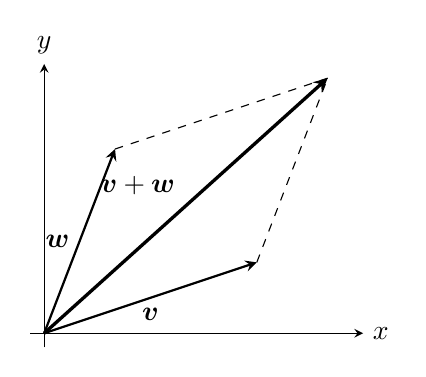
\begin{tikzpicture}[scale=0.9,>=stealth]
			\draw[->] (-0.2,0) -- (4.5,0) node[right] {$x$};
			\draw[->] (0,-0.2) -- (0,3.8) node[above] {$y$};
			\draw[->,thick] (0,0) -- (3,1) node[midway,below] {$\bm{v}$};
			\draw[->,thick] (0,0) -- (1,2.6) node[midway,left] {$\bm{w}$};
			\draw[dashed] (3,1) -- (4,3.6);
			\draw[dashed] (1,2.6) -- (4,3.6);
			\draw[->,very thick] (0,0) -- (4,3.6) node[midway,above left] {$\bm{v}+\bm{w}$};
		\end{tikzpicture}
		
		图 1：向量加法与线性组合的几何直观
	\end{center}
	
	再加入第三个不在该平面内的向量 $\bm{w}$，所有
	\begin{equation}\label{eq:1.9}
	c\bm{u}+d\bm{v}+e\bm{w},\qquad c,d,e\in\R
	\end{equation}
	便会填满整个 $\R^3$。
	
	如果第三个向量满足
	\begin{equation}\label{eq:1.10}
	\bm{w}=c\bm{u}+d\bm{v},
	\end{equation}
	也就是说 $\bm{w}$ 本来就落在 $\bm{u}$ 与 $\bm{v}$ 张成的平面内，那么三者的所有线性组合仍然只是原来那个平面，这时我们称 $\bm{u},\bm{v},\bm{w}$ \textbf{线性相关}。要注意，线性相关并不是 $\bm{w}$ 一个向量的“问题”：只要系数 $c,d$ 不为零，把上面的等式移项，就能得到
	\begin{equation}\label{eq:1.11}
	\bm{u}=\frac{1}{c}\bm{w}-\frac{d}{c}\bm{v},
	\qquad
	\bm{v}=\frac{1}{d}\bm{w}-\frac{c}{d}\bm{u},
	\end{equation}
	即 $\bm{u}$ 和 $\bm{v}$ 同样可以分别由另外两个向量表示出来。说到底，线性相关的本质是三个向量中至少有一个是“多余的”，它能由其余向量组合得到。
	
	相反，如果 $\bm{w}$ 无法由 $\bm{u}$ 和 $\bm{v}$ 线性组合得到，那么 $\bm{u}$ 和 $\bm{v}$ 也同样无法由另外两个向量组合得到——否则把等式移项，就会推出 $\bm{w}$ 也能被组合出来，与假设矛盾。此时三个向量谁都不是多余的，我们称它们\textbf{线性无关}。
	
	从这里可以先记住一个非常重要的判断方式：若存在不全为零的系数 $x_1,\ldots,x_n$，使得判别方程
	\begin{equation}\label{eq:1.12}
	x_1\bm{v}_1+\cdots+x_n\bm{v}_n=\bm{0},
	\end{equation}
	则这些向量线性相关；
	
	对于该判别方程，如果只有
	\begin{equation}\label{eq:1.13}
	x_1=x_2=\cdots=x_n=0
	\end{equation}
	也就是它们的系数全部一起为 $0$ 时，线性组合才能得到零向量，则这些向量线性无关。
	\section{长度、角度与点积运算}

	前一章介绍了向量以及向量的线性运算和组合。让我们回到单个向量本身，看向量的长度、角度以及点积运算。先看平面上的情形。直角三角形的两条直角边为 $a$、$b$ 时，由勾股定理可知斜边长为 $\sqrt{a^2+b^2}$。把平面向量 $\bm{v}=(3,4)\trans$ 从原点画出来，它正好是一个直角三角形的斜边，两条直角边分别是 $3$ 与 $4$，所以它的长度是
	\begin{equation}\label{eq:2.1}
	\sqrt{3^2+4^2}=\sqrt{25}=5.
	\end{equation}

	三维向量只多走一步。例如 $\bm{v}=(1,2,2)\trans$，先在前两个分量所在的水平面内用一次勾股定理，得到 $\sqrt{1^2+2^2}=\sqrt{5}$，再以它和第三个分量 $2$ 为两条直角边用第二次：
	\begin{equation}\label{eq:2.2}
	\sqrt{(\sqrt{5})^2+2^2}=\sqrt{5+4}=\sqrt{9}=3.
	\end{equation}
	两次合起来，效果就是把三个分量各自平方、相加、再开方。照此推广，$n$ 维向量 $\bm{v}=(v_1,v_2,\ldots,v_n)\trans$ 的\textbf{长度}（也叫\textbf{范数}）定义为
	\begin{equation}\label{eq:2.3}
	\norm{\bm{v}}=\sqrt{v_1^2+v_2^2+\cdots+v_n^2}.
	\end{equation}
	长度总是非负的，并且只有零向量的长度为 $0$。把向量乘以数 $c$，长度就乘以 $c$ 的绝对值：
	\begin{equation}\label{eq:2.4}
	\norm{c\bm{v}}=|c|\,\norm{\bm{v}}.
	\end{equation}

	长度为 $1$ 的向量称为\textbf{单位向量}。只要 $\bm{v}\neq\bm{0}$，把它除以自己的长度，就得到与它同方向的单位向量：
	\begin{equation}\label{eq:2.5}
	\bm{u}=\frac{\bm{v}}{\norm{\bm{v}}}.
	\end{equation}
	例如 $\bm{v}=(3,4)\trans$ 的长度是 $5$，于是
	\begin{equation}\label{eq:2.6}
	\bm{u}=\frac{\bm{v}}{\norm{\bm{v}}}=\left(\frac{3}{5},\frac{4}{5}\right)\trans,
	\qquad
	\norm{\bm{u}}=\sqrt{\left(\frac{3}{5}\right)^2+\left(\frac{4}{5}\right)^2}=\sqrt{\frac{9+16}{25}}=1.
	\end{equation}

	有了长度，接下来的主角是两个向量之间的一种运算。先看一组具体的数：$\bm{v}=(1,2,3)\trans$ 与 $\bm{w}=(4,5,6)\trans$。把它们对应位置的分量两两相乘，再把三个乘积加起来：
	\begin{equation}\label{eq:2.7}
	1\times 4+2\times 5+3\times 6=4+10+18=32.
	\end{equation}
	这个“对应相乘再相加”的运算称为\textbf{点积}。一般地，两个 $n$ 维向量 $\bm{v}=(v_1,v_2,\ldots,v_n)\trans$ 与 $\bm{w}=(w_1,w_2,\ldots,w_n)\trans$ 的点积定义为
	\begin{equation}\label{eq:2.8}
	\bm{v}\cdot\bm{w}
	=v_1w_1+v_2w_2+\cdots+v_nw_n
	=\sum_{i=1}^{n}v_iw_i.
	\end{equation}
	点积的结果是一个标量，而不是向量。
	点积与长度直接相关：向量与自身做点积，得到的正是长度的平方，
	\begin{equation}\label{eq:2.9}
	\bm{v}\cdot\bm{v}=v_1^2+v_2^2+\cdots+v_n^2=\norm{\bm{v}}^2,
	\end{equation}
	也就是说 $\norm{\bm{v}}=\sqrt{\bm{v}\cdot\bm{v}}$。

	点积真正的重要性在于，它还藏着两个向量之间的夹角。下面用余弦定理把这一点完整推出来。设 $\bm{v}$ 与 $\bm{w}$ 都是非零向量，夹角为 $\theta$。把它们从同一点画出，两个终点之间连线所对应的向量是 $\bm{v}-\bm{w}$，三者构成一个三角形。余弦定理给出
	\begin{equation}\label{eq:2.10}
	\norm{\bm{v}-\bm{w}}^2=\norm{\bm{v}}^2+\norm{\bm{w}}^2-2\norm{\bm{v}}\norm{\bm{w}}\cos\theta.
	\end{equation}
	等式左边可以用点积逐步展开。点积对加减法可以像普通乘法一样逐项展开，因为它本来就是按分量相乘再相加；展开过程是
	\begin{equation}\label{eq:2.11}
	\begin{aligned}
	\norm{\bm{v}-\bm{w}}^2
	&=(\bm{v}-\bm{w})\cdot(\bm{v}-\bm{w})\\
	&=\bm{v}\cdot(\bm{v}-\bm{w})-\bm{w}\cdot(\bm{v}-\bm{w})\\
	&=\bm{v}\cdot\bm{v}-\bm{v}\cdot\bm{w}-\bm{w}\cdot\bm{v}+\bm{w}\cdot\bm{w}\\
	&=\norm{\bm{v}}^2-2\,\bm{v}\cdot\bm{w}+\norm{\bm{w}}^2,
	\end{aligned}
	\end{equation}
	最后一步用到了 $\bm{v}\cdot\bm{v}=\norm{\bm{v}}^2$ 与点积的交换律 $\bm{v}\cdot\bm{w}=\bm{w}\cdot\bm{v}$（分量相乘的顺序不影响乘积），所以中间两项合在了一起。把这个结果与余弦定理对比，两边相同的 $\norm{\bm{v}}^2+\norm{\bm{w}}^2$ 约去，剩下
	\begin{equation}\label{eq:2.12}
	-2\,\bm{v}\cdot\bm{w}=-2\norm{\bm{v}}\norm{\bm{w}}\cos\theta,
	\end{equation}
再约去 $-2$，得到点积的几何公式~\eqref{eq:2.13}
	\begin{equation}\label{eq:2.13}
	\bm{v}\cdot\bm{w}=\norm{\bm{v}}\norm{\bm{w}}\cos\theta,
	\end{equation}
也就是夹角公式~\eqref{eq:2.14}
	\begin{equation}\label{eq:2.14}
	\cos\theta=\frac{\bm{v}\cdot\bm{w}}{\norm{\bm{v}}\norm{\bm{w}}}.
	\end{equation}

	回到刚才的数字例子，可以真正算出 $\bm{v}=(1,2,3)\trans$ 与 $\bm{w}=(4,5,6)\trans$ 的夹角。先算两个长度：
	\begin{equation}\label{eq:2.15}
	\norm{\bm{v}}=\sqrt{1^2+2^2+3^2}=\sqrt{14},
	\qquad
	\norm{\bm{w}}=\sqrt{4^2+5^2+6^2}=\sqrt{77},
	\end{equation}
再代入夹角公式~\eqref{eq:2.14}，点积已经在前面算出是 $32$：
	\begin{equation}\label{eq:2.16}
	\cos\theta=\frac{32}{\sqrt{14}\sqrt{77}}=\frac{32}{\sqrt{1078}}\approx 0.975,
	\qquad
	\theta\approx 12.9^\circ.
	\end{equation}

	由于长度总是非负的，点积的符号完全由 $\cos\theta$ 的符号决定：
	\begin{itemize}
		\item $\bm{v}\cdot\bm{w}>0$ 当且仅当 $\cos\theta>0$，此时夹角 $\theta$ 是锐角（$0\le\theta<90^\circ$）；
		\item $\bm{v}\cdot\bm{w}=0$ 当且仅当 $\cos\theta=0$，此时 $\theta=90^\circ$；
		\item $\bm{v}\cdot\bm{w}<0$ 当且仅当 $\cos\theta<0$，此时夹角 $\theta$ 是钝角（$90^\circ<\theta\le 180^\circ$）。
	\end{itemize}

	第二种情形有一个专门的名字：当
	\begin{equation}\label{eq:2.17}
	\bm{v}\cdot\bm{w}=0
	\end{equation}
	时，称 $\bm{v}$ 与 $\bm{w}$ \textbf{正交}，也就是互相垂直。零向量与任何向量的点积都是 $0$，所以它被视为与任何向量正交。正交还可以用本章开头的勾股定理来检验：由 $\norm{\bm{v}+\bm{w}}^2=\norm{\bm{v}}^2+2\,\bm{v}\cdot\bm{w}+\norm{\bm{w}}^2$ 可知，$\bm{v}$ 与 $\bm{w}$ 正交当且仅当
	\begin{equation}\label{eq:2.18}
	\norm{\bm{v}+\bm{w}}^2=\norm{\bm{v}}^2+\norm{\bm{w}}^2,
	\end{equation}
	这正是“直角三角形斜边的平方等于两直角边平方之和”的向量形式。正交是后面投影、最小二乘、正交基以及许多数值算法的基础。

夹角公式~\eqref{eq:2.14} 还带来两条经常用到的长度估计。因为 $|\cos\theta|\le 1$，对几何公式~\eqref{eq:2.13} 两边取绝对值就得到
	\begin{equation}\label{eq:2.19}
	|\bm{v}\cdot\bm{w}|=\norm{\bm{v}}\norm{\bm{w}}\,|\cos\theta|\le\norm{\bm{v}}\norm{\bm{w}}.
	\end{equation}
	这称为 \textbf{Cauchy--Schwarz 不等式}：点积的绝对值不会超过两个向量长度的乘积。若 $\bm{v}$ 或 $\bm{w}$ 是零向量，不等式两边都是 $0$，自然成立；等号成立当且仅当 $|\cos\theta|=1$，也就是两个向量共线。

	由它还可以推出\textbf{三角不等式}。先把 $\norm{\bm{v}+\bm{w}}^2$ 逐步展开：
	\begin{equation}\label{eq:2.20}
	\begin{aligned}
	\norm{\bm{v}+\bm{w}}^2
	&=(\bm{v}+\bm{w})\cdot(\bm{v}+\bm{w})\\
	&=\bm{v}\cdot\bm{v}+\bm{v}\cdot\bm{w}+\bm{w}\cdot\bm{v}+\bm{w}\cdot\bm{w}\\
	&=\norm{\bm{v}}^2+2\,\bm{v}\cdot\bm{w}+\norm{\bm{w}}^2.
	\end{aligned}
	\end{equation}
	对中间的点积用 Cauchy--Schwarz 不等式，$\bm{v}\cdot\bm{w}\le|\bm{v}\cdot\bm{w}|\le\norm{\bm{v}}\norm{\bm{w}}$，于是
	\begin{equation}\label{eq:2.21}
	\norm{\bm{v}+\bm{w}}^2
	\le\norm{\bm{v}}^2+2\norm{\bm{v}}\norm{\bm{w}}+\norm{\bm{w}}^2
	=\bigl(\norm{\bm{v}}+\norm{\bm{w}}\bigr)^2.
	\end{equation}
	两边都是非负实数，开平方后得到
	\begin{equation}\label{eq:2.22}
	\norm{\bm{v}+\bm{w}}\le\norm{\bm{v}}+\norm{\bm{w}}.
	\end{equation}
	几何上这正是三角形的基本事实：任何一边的长度不超过另外两边长度之和。
	\section{矩阵}
	
	考虑一个简单的二元一次方程组：
	\begin{equation}\label{eq:3.1}
	x+2y=4,
	\qquad
	3x+4y=10,
	\end{equation}
	未知数 $x,y$ 其实只是占位的符号，真正参与运算的是它们的系数和右端的数。把系数按原来的位置抄出来，排成一张矩形数表：
	\begin{equation}\label{eq:3.2}
	\begin{bmatrix}
		1&2\\
		3&4
	\end{bmatrix}.
	\end{equation}
	这样的矩形数表就称为\textbf{矩阵}，这里的矩阵是2行2列的，我们也就称它为 $2\times 2$ 矩阵。同理，当它有 $m$ 行 $n$ 列时，称为一个 $m\times n$ 矩阵。
	
	方程增多、未知数增多时，数表只是随之变大。例如在上面两个方程之后再添一个方程 $5x+6y=16$，三个方程的系数排成的矩阵是
	\begin{equation}\label{eq:3.3}
	A=
	\begin{bmatrix}
		1&2\\
		3&4\\
		5&6
	\end{bmatrix},
	\end{equation}
	它有 $3$ 行 $2$ 列，称为一个 $3\times 2$ 矩阵。右端的三个数 $4,10,16$ 也排成一列，记作列向量 $\bm{b}=(4,10,16)\trans$。
	
	不过，虽然这里的矩阵我们是看每一行的方程系数并塞进去，矩阵也是一行一行组成的，但如果从竖列的角度来看，我们不难发现矩阵就是把许多列向量并排放在一起。把 $A$ 按列拆开，可以写为
	\begin{equation}\label{eq:3.4}
	A=
	\begin{bmatrix}
		\bm{a}_1 & \bm{a}_2
	\end{bmatrix},
	\qquad
	\bm{a}_1=
	\begin{bmatrix}
		1\\3\\5
	\end{bmatrix},
	\quad
	\bm{a}_2=
	\begin{bmatrix}
		2\\4\\6
	\end{bmatrix}.
	\end{equation}
	
	这里我们可以很清晰的看出来，矩阵$A$可以看作是$a_1$与$a_2$两个列向量组合排列起来而形成的。（help，这里帮我将这个a1与a2格式规范一下，进行加粗处理）之前我们讲过，线性组合是向量最重要的运算之一，矩阵我们可以认为是多个向量叠加在一起的，因此矩阵与向量之间的乘法也是符合线性组合的规则的。设
	\begin{equation}\label{eq:3.5}
	\bm{x}=
	\begin{bmatrix}
		x_1\\x_2
	\end{bmatrix},
	\end{equation}
	则矩阵与向量的乘积
	\begin{equation}\label{eq:3.6}
	A\bm{x}
	=
	\begin{bmatrix}
		1&2\\
		3&4\\
		5&6
	\end{bmatrix}
	\begin{bmatrix}
		x_1\\x_2
	\end{bmatrix}
	\end{equation}
	规定为
	\begin{equation}\label{eq:3.7}
	\boxed{A\bm{x}=x_1\bm{a}_1+x_2\bm{a}_2.}
	\end{equation}
	也就是说，$A\bm{x}$ 的计算过程我们可以认为是矩阵 $A$ 的列向量重新进行线性组合，而 $\bm{x}$ 的各个分量正是组合系数。这就是后文反复使用的列图像。
	
	另一方面，也可以把 $A$ 按行拆开。把 $A$ 的行向量记作
	\begin{equation}\label{eq:3.8}
	\bm{r}_1\trans,\bm{r}_2\trans,\bm{r}_3\trans
	\end{equation}
	其中 $\bm{r}_i\trans$ 表示第 $i$ 行，$\bm{r}_i$ 是把这一行竖起来得到的列向量。点积 $\bm{v}\cdot\bm{w}$ 也可以写成 $\bm{v}\trans\bm{w}$ 的形式；用这个记号就有
	\begin{equation}\label{eq:3.9}
	A\bm{x}
	=
	\begin{bmatrix}
		\bm{r}_1\trans\bm{x}\\
		\bm{r}_2\trans\bm{x}\\
		\vdots\\
		\bm{r}_m\trans\bm{x}
	\end{bmatrix}.
	\end{equation}
	因此矩阵乘向量也可以理解为：\textbf{每一行分别与输入向量做一次点积。}
	
	两种看法到底一不一样，取一个具体的 $\bm{x}$ 完整算一遍就知道了。取
	\begin{equation}\label{eq:3.10}
	\bm{x}=
	\begin{bmatrix}
		2\\1
	\end{bmatrix},
	\end{equation}
	即 $x_1=2$，$x_2=1$。先按列看：分别算出两列的倍数
	\begin{equation}\label{eq:3.11}
	2\bm{a}_1
	=
	2
	\begin{bmatrix}
		1\\3\\5
	\end{bmatrix}
	=
	\begin{bmatrix}
		2\\6\\10
	\end{bmatrix},
	\qquad
	1\bm{a}_2
	=
	\begin{bmatrix}
		2\\4\\6
	\end{bmatrix},
	\end{equation}
	再把它们相加。于是 $A\bm{x}=2\bm{a}_1+1\bm{a}_2$，即
	\begin{equation}\label{eq:3.12}
	\begin{bmatrix}
		2\\6\\10
	\end{bmatrix}
	+
	\begin{bmatrix}
		2\\4\\6
	\end{bmatrix}
	=
	\begin{bmatrix}
		2+2\\6+4\\10+6
	\end{bmatrix}
	=
	\begin{bmatrix}
		4\\10\\16
	\end{bmatrix}.
	\end{equation}
	再按行看。三行分别是 $\bm{r}_1\trans=(1,2)$，$\bm{r}_2\trans=(3,4)$，$\bm{r}_3\trans=(5,6)$，逐行与 $\bm{x}$ 做点积。第一行：
	\begin{equation}\label{eq:3.13}
	\bm{r}_1\trans\bm{x}=1\cdot2+2\cdot1=4.
	\end{equation}
	第二行：
	\begin{equation}\label{eq:3.14}
	\bm{r}_2\trans\bm{x}=3\cdot2+4\cdot1=10.
	\end{equation}
	第三行：
	\begin{equation}\label{eq:3.15}
	\bm{r}_3\trans\bm{x}=5\cdot2+6\cdot1=16.
	\end{equation}
	三个分量依次是 $4,10,16$，拼起来正是
	\begin{equation}\label{eq:3.16}
	A\bm{x}=
	\begin{bmatrix}
		4\\10\\16
	\end{bmatrix},
	\end{equation}
	与按列看的结果完全相同。
	
	这不是巧合，逐分量对照一下就清楚了。按列看时，组合 $x_1\bm{a}_1+x_2\bm{a}_2$ 的第 $i$ 个分量，是各列的第 $i$ 个分量分别乘上系数再相加，即 $x_1a_{i1}+x_2a_{i2}$；按行看时，第 $i$ 行 $(a_{i1},a_{i2})$ 与 $\bm{x}$ 的点积是 $a_{i1}x_1+a_{i2}x_2$。两者是同一批乘法和加法，只是分组顺序不同，所以必然相等。比如第一个分量，按列看是 $2\cdot1+1\cdot2=4$，按行看是 $1\cdot2+2\cdot1=4$，连中间步骤都对得上。
	
	于是同一个 $A\bm{x}$ 有两种完全等价但关注点不同的理解：
	\begin{enumerate}
		\item \textbf{按列看：} $A\bm{x}$ 是各列的线性组合；
		\item \textbf{按行看：} $A\bm{x}$ 的每个分量是某一行与 $\bm{x}$ 的点积。
	\end{enumerate}
	只做数值计算时，“行乘列”已经足够；但要理解线性代数的结构，“列的线性组合”往往更重要。
	
	\subsection{从 \texorpdfstring{$A\bm{x}$}{Ax} 到 \texorpdfstring{$A\bm{x}=\bm{b}$}{Ax=b}}
	
	若 $\bm{x}$ 已知，那么 $A\bm{x}$ 只是一次顺向计算，就像刚才取 $\bm{x}=(2,1)\trans$ 算出 $(4,10,16)\trans$ 那样。线性代数真正关心的经典问题通常反过来：给定 $A$ 和 $\bm{b}$，寻找
	\begin{equation}\label{eq:3.17}
	A\bm{x}=\bm{b}
	\end{equation}
	的解 $\bm{x}$。
	
	从列向量的角度看，这个问题等价于：\textbf{能否找到一组系数，使 $A$ 的列向量线性组合后恰好得到 $\bm{b}$？}继续用上面那组数来试：给定同样的 $A$ 和 $\bm{b}=(4,10,16)\trans$，要找 $x_1,x_2$ 使得
	\begin{equation}\label{eq:3.18}
	x_1
	\begin{bmatrix}
		1\\3\\5
	\end{bmatrix}
	+x_2
	\begin{bmatrix}
		2\\4\\6
	\end{bmatrix}
	=
	\begin{bmatrix}
		4\\10\\16
	\end{bmatrix}.
	\end{equation}
	按分量写出来，就是三个方程
	\begin{equation}\label{eq:3.19}
	x_1+2x_2=4,
	\qquad
	3x_1+4x_2=10,
	\qquad
	5x_1+6x_2=16.
	\end{equation}
	用通常的消元方法处理前两个方程：第二式减去第一式的 $3$ 倍，得 $-2x_2=-2$，所以 $x_2=1$；代回第一式，得 $x_1=2$。解必须同时满足全部三个方程，因此还要代入第三个方程检验：$5\cdot2+6\cdot1=16$，恰好成立。所以 $\bm{x}=(2,1)\trans$ 确实是解——它就是上一节按列组合时用过的那组系数。
	
	一般地，若
	\begin{equation}\label{eq:3.20}
	A=
	\begin{bmatrix}
		\bm{a}_1&\cdots&\bm{a}_n
	\end{bmatrix},
	\end{equation}
	那么
	\begin{equation}\label{eq:3.21}
	A\bm{x}=\bm{b}
	\iff
	x_1\bm{a}_1+\cdots+x_n\bm{a}_n=\bm{b}.
	\end{equation}
	因此，求解线性方程组和寻找线性组合，本质上是同一件事。
	
	对于可逆方阵 $A$，解可以形式地写成
	\begin{equation}\label{eq:3.22}
	\bm{x}=A^{-1}\bm{b}.
	\end{equation}
	这里的 $A^{-1}$ 称为 $A$ 的\textbf{逆矩阵}，暂时只需把它理解成“从输出 $\bm{b}$ 恢复输入 $\bm{x}$ 的逆变换”；实际求解大型方程组时并不会先显式算出 $A^{-1}$，这一点留到消元与分解时再谈。
	
	\subsection{从 \texorpdfstring{$A\bm{x}=\bm{0}$}{Ax=0} 看线性相关}
	
	矩阵语言还能把第 1 章的线性相关问题写得非常紧凑。第 1 章的判别方程问的是：是否存在不全为零的系数，使线性组合等于零向量。若
	\begin{equation}\label{eq:3.23}
	A=
	\begin{bmatrix}
		\bm{a}_1&\bm{a}_2&\cdots&\bm{a}_n
	\end{bmatrix},
	\end{equation}
	则
	\begin{equation}\label{eq:3.24}
	A\bm{x}=\bm{0}
	\end{equation}
	等价于
	\begin{equation}\label{eq:3.25}
	x_1\bm{a}_1+x_2\bm{a}_2+\cdots+x_n\bm{a}_n=\bm{0}.
	\end{equation}
	因此：
	\begin{itemize}
		\item 如果 $A\bm{x}=\bm{0}$ 只有零解 $\bm{x}=\bm{0}$，那么这些列向量线性无关；
		\item 如果存在非零解 $\bm{x}\neq\bm{0}$，那么这些列向量线性相关。
	\end{itemize}
	
	两种情况各算一个例子。先取只有两列的 $A$，问 $A\bm{x}=\bm{0}$ 即
	\begin{equation}\label{eq:3.26}
	x_1
	\begin{bmatrix}
		1\\3\\5
	\end{bmatrix}
	+x_2
	\begin{bmatrix}
		2\\4\\6
	\end{bmatrix}
	=
	\begin{bmatrix}
		0\\0\\0
	\end{bmatrix}
	\end{equation}
	有没有非零解。按分量写出来：
	\begin{equation}\label{eq:3.27}
	x_1+2x_2=0,
	\qquad
	3x_1+4x_2=0,
	\qquad
	5x_1+6x_2=0.
	\end{equation}
	第二式减去第一式的 $3$ 倍，得 $-2x_2=0$，即 $x_2=0$；代回第一式得 $x_1=0$。方程组只有零解 $\bm{x}=\bm{0}$，所以这两列线性无关。
	
	再添上第三列 $\bm{a}_3=(3,7,11)\trans$。先看一个事实：
	\begin{equation}\label{eq:3.28}
	\bm{a}_1+\bm{a}_2
	=
	\begin{bmatrix}
		1+2\\3+4\\5+6
	\end{bmatrix}
	=
	\begin{bmatrix}
		3\\7\\11
	\end{bmatrix}
	=\bm{a}_3,
	\end{equation}
	即 $\bm{a}_3$ 能由前两列组合得到。移项可得 $\bm{a}_1+\bm{a}_2-\bm{a}_3=\bm{0}$，也就是说 $\bm{x}=(1,1,-1)\trans$ 满足
	\begin{equation}\label{eq:3.29}
	\begin{bmatrix}
		1\\3\\5
	\end{bmatrix}
	+
	\begin{bmatrix}
		2\\4\\6
	\end{bmatrix}
	-
	\begin{bmatrix}
		3\\7\\11
	\end{bmatrix}
	=
	\begin{bmatrix}
		1+2-3\\3+4-7\\5+6-11
	\end{bmatrix}
	=
	\begin{bmatrix}
		0\\0\\0
	\end{bmatrix}.
	\end{equation}
	组合系数 $1,1,-1$ 不全为零，所以 $\bm{x}=(1,1,-1)\trans$ 是一个非零解，这三列线性相关。这正是第 1 章说的“第三个向量落在前两个向量张成的平面内，是多余的”。
	
	对于方阵，这还会和矩阵是否可逆直接联系起来：列向量线性无关时，$A\bm{x}=\bm{0}$ 只有零解；列向量线性相关时就会出现非零解，矩阵不再可逆。这个联系后面还会被系统地展开。
	\section{线性方程、消元与矩阵分解}
	
	第 3 章已经把方程
	\begin{equation}\label{eq:4.1}
	A\bm{x}=\bm{b}
	\end{equation}
	理解为“用 $A$ 的列向量线性组合出 $\bm{b}$，组合系数就是 $\bm{x}$”。但当时只回答了“解是什么”，还没有回答“怎样算”。这一章就动手解决两个更进一步的问题：怎样一步一步把 $\bm{x}$ 求出来，以及求解过程反过来能告诉我们矩阵 $A$ 的哪些结构。核心工具只有一个——高斯消元；而它走完全程之后，会自然长成矩阵分解。
	
	\subsection{行图像、列图像与高斯消元}
	
	从一个具体的方程组开始。取
	\begin{equation}\label{eq:4.2}
	A=
	\begin{bmatrix}
		1&-2\\
		3&2
	\end{bmatrix},
	\qquad
	\bm{x}=
	\begin{bmatrix}
		x\\y
	\end{bmatrix},
	\qquad
	\bm{b}=
	\begin{bmatrix}
		1\\11
	\end{bmatrix},
	\end{equation}
	则 $A\bm{x}=\bm{b}$ 就是
	\begin{equation}\label{eq:4.3}
	\begin{cases}
		x-2y=1,\\
		3x+2y=11.
	\end{cases}
	\end{equation}
	同一个方程组有两种看法。按行看，每个方程在平面上给出一条直线，两条直线的交点就是解；按列看，是在为 $A$ 的两列寻找组合系数：
	\begin{equation}\label{eq:4.4}
	x
	\begin{bmatrix}
		1\\3
	\end{bmatrix}
	+y
	\begin{bmatrix}
		-2\\2
	\end{bmatrix}
	=
	\begin{bmatrix}
		1\\11
	\end{bmatrix}.
	\end{equation}
	二维时行图像很直观；进入高维以后，列向量的线性组合往往更加直接。但两种看法找到的必须是同一组 $x,y$。
	
	求解这样的方程组，最基本的方法是\textbf{高斯消元}：通过行与行之间的加减，把方程组逐步变成上三角形状，再从下往上把未知量逐个解出来。先用上面的例子把全过程走一遍。
	
	第一步是消元：用第一个方程消去第二个方程里的 $x$。第一个方程中 $x$ 的系数 $1$ 称为第一个\textbf{主元}（pivot），它是这一步消元的基准，必须非零才能用。第二个方程中 $x$ 的系数是 $3$，所以用第二个方程减去第一个方程的 $3$ 倍：
	\begin{equation}\label{eq:4.5}
	(3x+2y)-3(x-2y)=11-3\times 1.
	\end{equation}
	左边展开：$3x$ 与 $-3x$ 抵消，$2y-3\times(-2y)=2y+6y=8y$；右边是 $11-3=8$。方程组变成
	\begin{equation}\label{eq:4.6}
	\begin{cases}
		x-2y=1,\\
		8y=8.
	\end{cases}
	\end{equation}
	第一个方程原封不动，第二个方程里的 $x$ 被消掉了。此时系数矩阵是
	\begin{equation}\label{eq:4.7}
	U=
	\begin{bmatrix}
		1&-2\\
		0&8
	\end{bmatrix},
	\end{equation}
	主对角线以下全是零，这样的矩阵称为\textbf{上三角矩阵}。两个主元 $1$ 和 $8$ 就站在对角线上。
	
	第二步是\textbf{回代}：从最后一个方程开始，逐行向上求解。由 $8y=8$ 得 $y=1$；代回第一个方程，
	\begin{equation}\label{eq:4.8}
	x=1+2y=1+2\times 1=3.
	\end{equation}
	检验一下：$3-2\times 1=1$，$3\times 3+2\times 1=11$，两个方程都满足。解就是 $(x,y)=(3,1)$。
	
把这套动作写成一般公式~\eqref{eq:4.9}。设第一个主元 $a_{11}\neq 0$，要消去第 $i$ 行中的 $a_{i1}$，先算\textbf{乘子}
	\begin{equation}\label{eq:4.9}
	\ell_{i1}=\frac{a_{i1}}{a_{11}},
	\end{equation}
	即“要消掉的元素”除以主元，然后做行变换
	\begin{equation}\label{eq:4.10}
	\text{第 }i\text{ 行}
	\leftarrow
	\text{第 }i\text{ 行}
	-
	\ell_{i1}\,\text{第 }1\text{ 行}.
	\end{equation}
	上面的例子正是 $\ell_{21}=\dfrac{3}{1}=3$。第一列处理完后，在主元右下方剩下的子矩阵里重复同样的事：找第二个主元，消去它下方的元素，再找第三个主元，直到方程组变成
	\begin{equation}\label{eq:4.11}
	U\bm{x}=\bm{c},
	\end{equation}
	其中 $\bm{c}$ 是 $\bm{b}$ 跟着做完同样行变换后的结果。最后回代，从最后一个未知量一路解回第一个。
	
	主元必须非零，因为它要做除数。若某一步主元位置上是 $0$，而它下方还有非零元素，就交换两行，把非零元素换到主元位置上。若整列在当前主元位置及其以下全是零，这一列就无法产生新的主元，方程组会出现可以任意取值的未知量（\textbf{自由变量}），矩阵的秩也会小于列数。主元究竟出现在哪里、出现几个，后面关于秩和子空间的讨论会系统地回答。
	
	\subsection{消元矩阵与置换矩阵}
	
	每一次行消元都可以写成一次矩阵乘法。若要用第 $j$ 行消去第 $i$ 行中的元素，记对应的\textbf{消元矩阵}为 $E_{ij}$：把单位矩阵 $I$ 的 $(i,j)$ 位置换成乘子的相反数 $-\ell_{ij}$，其余不动，则
	\begin{equation}\label{eq:4.12}
	E_{ij}A
	\end{equation}
	就是完成该次行变换后的矩阵。
	
	还用上面的例子。“第二行减去 $3$ 倍第一行”对应
	\begin{equation}\label{eq:4.13}
	E_{21}=
	\begin{bmatrix}
		1&0\\
		-3&1
	\end{bmatrix}.
	\end{equation}
	真的把它乘到 $A$ 上看看：
	\begin{equation}\label{eq:4.14}
	E_{21}A
	=
	\begin{bmatrix}
		1&0\\
		-3&1
	\end{bmatrix}
	\begin{bmatrix}
		1&-2\\
		3&2
	\end{bmatrix}
	=
	\begin{bmatrix}
		1&-2\\
		0&8
	\end{bmatrix}
	=U.
	\end{equation}
	逐个元素核对：第一行是 $1$ 倍原第一行加 $0$ 倍原第二行，原封不动；第二行第一列是 $-3\times 1+1\times 3=0$，正是要消掉的位置；第二行第二列是 $-3\times(-2)+1\times 2=8$，正是新主元。矩阵乘法忠实地执行了手算的那一步消元。
	
	方程右端必须做完全相同的行变换：
	\begin{equation}\label{eq:4.15}
	E_{21}\bm{b}
	=
	\begin{bmatrix}
		1&0\\
		-3&1
	\end{bmatrix}
	\begin{bmatrix}
		1\\11
	\end{bmatrix}
	=
	\begin{bmatrix}
		1\\8
	\end{bmatrix}
	=\bm{c}.
	\end{equation}
	于是 $E_{21}A\bm{x}=E_{21}\bm{b}$ 正好就是上三角系统 $U\bm{x}=\bm{c}$。为了不让同样的变换做两遍，实际消元时把 $\bm{b}$ 作为附加的一列接在 $A$ 右边，拼成\textbf{增广矩阵}
	\begin{equation}\label{eq:4.16}
	[A\mid \bm{b}],
	\end{equation}
	对整块一起做行变换。若消元需要多步，就有多个消元矩阵依次左乘：
	\begin{equation}\label{eq:4.17}
	E_k\cdots E_2E_1A=U,
	\qquad
	E_k\cdots E_2E_1\bm{b}=\bm{c}.
	\end{equation}
	注意书写顺序：先执行的那一步离 $A$ 最近。
	
	交换两行也有对应的矩阵。把单位矩阵 $I$ 的第 $i,j$ 两行互换，得到的矩阵称为\textbf{置换矩阵}；左乘它，就会交换矩阵的第 $i,j$ 两行。二维的例子：
	\begin{equation}\label{eq:4.18}
	P=
	\begin{bmatrix}
		0&1\\
		1&0
	\end{bmatrix},
	\qquad
	P
	\begin{bmatrix}
		x\\y
	\end{bmatrix}
	=
	\begin{bmatrix}
		y\\x
	\end{bmatrix},
	\end{equation}
	两个分量真的被交换了。置换矩阵满足
	\begin{equation}\label{eq:4.19}
	P^{-1}=P\trans.
	\end{equation}
	原因是：把同一次交换再做一遍就回到了原来的排列，所以这个例子里 $PP=I$，$P$ 是它自己的逆；而 $P$ 本身又是对称的，$P\trans=P$，合起来就是 $P^{-1}=P\trans$。
	
	\subsection{矩阵乘法的结构}
	
	消元矩阵已经用到了矩阵乘法，现在把它本身的结构看清楚。设 $A\in\R^{m\times n}$，$B\in\R^{n\times p}$，则乘积 $AB$ 有定义，并且
	\begin{equation}\label{eq:4.20}
	AB\in\R^{m\times p}.
	\end{equation}
	内侧的两个 $n$ 必须相同，结果的形状取外侧的 $m$ 与 $p$。
	
	最熟悉的定义是“行乘列”：
	\begin{equation}\label{eq:4.21}
	(AB)_{ij}
	=
	\sum_{k=1}^{n}a_{ik}b_{kj},
	\end{equation}
	即 $AB$ 的第 $(i,j)$ 个元素，是 $A$ 的第 $i$ 行与 $B$ 的第 $j$ 列的点积。取一对具体的矩阵算到底：
	\begin{equation}\label{eq:4.22}
	A=
	\begin{bmatrix}
		1&2\\
		3&4
	\end{bmatrix},
	\qquad
	B=
	\begin{bmatrix}
		5&6\\
		7&8
	\end{bmatrix}.
	\end{equation}
	四个元素分别是
	\begin{equation}\label{eq:4.23}
	\begin{aligned}
		(AB)_{11}&=1\times5+2\times7=19, &
		(AB)_{12}&=1\times6+2\times8=22,\\
		(AB)_{21}&=3\times5+4\times7=43, &
		(AB)_{22}&=3\times6+4\times8=50,
	\end{aligned}
	\end{equation}
	所以
	\begin{equation}\label{eq:4.24}
	AB=
	\begin{bmatrix}
		19&22\\
		43&50
	\end{bmatrix}.
	\end{equation}
	
	行乘列是算法，理解结构还要看列。若
	\begin{equation}\label{eq:4.25}
	B=
	\begin{bmatrix}
		\bm{b}_1&\bm{b}_2&\cdots&\bm{b}_p
	\end{bmatrix},
	\end{equation}
	则
	\begin{equation}\label{eq:4.26}
	AB=
	\begin{bmatrix}
		A\bm{b}_1&A\bm{b}_2&\cdots&A\bm{b}_p
	\end{bmatrix}.
	\end{equation}
	$A$ 逐列作用在 $B$ 上，乘积的每一列都是 $A$ 的列向量的线性组合——第 3 章的列图像在这里原样适用。反过来，也可以把 $AB$ 的第 $i$ 行看成 $A$ 的第 $i$ 行乘上整个 $B$。
	
	还有第三种看法。把 $A$ 按列拆开、$B$ 按行拆开：
	\begin{equation}\label{eq:4.27}
	A=
	\begin{bmatrix}
		\bm{a}_1&\cdots&\bm{a}_n
	\end{bmatrix},
	\qquad
	B=
	\begin{bmatrix}
		\bm{r}_1\trans\\
		\vdots\\
		\bm{r}_n\trans
	\end{bmatrix},
	\end{equation}
	则
	\begin{equation}\label{eq:4.28}
	AB
	=
	\bm{a}_1\bm{r}_1\trans+
	\bm{a}_2\bm{r}_2\trans+
	\cdots+
	\bm{a}_n\bm{r}_n\trans.
	\end{equation}
	每一项都是“列向量乘行向量”，结果是一个\textbf{秩一矩阵}：它的各列都是 $\bm{a}_i$ 的倍数，互相平行。用上面那对矩阵验证一下：
	\begin{equation}\label{eq:4.29}
	\begin{bmatrix}
		1\\3
	\end{bmatrix}
	(5,6)
	+
	\begin{bmatrix}
		2\\4
	\end{bmatrix}
	(7,8)
	=
	\begin{bmatrix}
		5&6\\
		15&18
	\end{bmatrix}
	+
	\begin{bmatrix}
		14&16\\
		28&32
	\end{bmatrix}
	=
	\begin{bmatrix}
		19&22\\
		43&50
	\end{bmatrix},
	\end{equation}
	与行乘列的结果完全相同。这个写法在矩阵分解中还会反复出现。
	
	运算律方面，矩阵乘法满足结合律
	\begin{equation}\label{eq:4.30}
	(AB)C=A(BC),
	\end{equation}
	以及对加法的分配律，但一般\textbf{不满足交换律}：
	\begin{equation}\label{eq:4.31}
	AB\neq BA.
	\end{equation}
	还用上面那对矩阵：
	\begin{equation}\label{eq:4.32}
	BA=
	\begin{bmatrix}
		5&6\\
		7&8
	\end{bmatrix}
	\begin{bmatrix}
		1&2\\
		3&4
	\end{bmatrix}
	=
	\begin{bmatrix}
		23&34\\
		31&46
	\end{bmatrix}
	\neq AB.
	\end{equation}
	甚至有时 $AB$ 有定义而 $BA$ 的维数根本对不上。所以矩阵乘积中因子的顺序不能随意调换，这也是上一节里消元矩阵必须按顺序书写的原因。
	
	\subsection{逆矩阵与 Gauss--Jordan 消元}
	
	对于方阵 $A$，若存在矩阵 $A^{-1}$ 使
	\begin{equation}\label{eq:4.33}
	A^{-1}A=AA^{-1}=I,
	\end{equation}
	则称 $A$ \textbf{可逆}，$A^{-1}$ 称为它的\textbf{逆矩阵}。此时
	\begin{equation}\label{eq:4.34}
	A\bm{x}=\bm{b}
	\end{equation}
	有唯一解
	\begin{equation}\label{eq:4.35}
	\bm{x}=A^{-1}\bm{b}.
	\end{equation}
不过公式~\eqref{eq:4.35} 的作用主要是说明结构；实际计算中通常不会先把逆矩阵算出来再乘 $\bm{b}$。第 3 章答应过解释原因，答案就是前面的消元：对具体的 $\bm{b}$ 直接消元，比求出整个 $A^{-1}$ 再相乘省事得多。
	
	判断可逆性最直接的工具是齐次方程。若存在非零向量 $\bm{x}\neq\bm{0}$ 满足
	\begin{equation}\label{eq:4.36}
	A\bm{x}=\bm{0},
	\end{equation}
	那么 $A$ 不可能可逆——否则两边左乘 $A^{-1}$，会推出 $\bm{x}=A^{-1}\bm{0}=\bm{0}$，矛盾。联系第 3 章的结论：$A\bm{x}=\bm{0}$ 有非零解，正是列向量线性相关。因此对方阵来说，下面三件事是同一件事：$A$ 可逆；齐次方程只有零解；$A$ 的列向量线性无关。
	
	看一个不可逆的例子：
	\begin{equation}\label{eq:4.37}
	A=
	\begin{bmatrix}
		1&2\\
		2&4
	\end{bmatrix},
	\end{equation}
	第二列是第一列的 $2$ 倍，列向量线性相关。取 $\bm{x}=(2,-1)\trans$：
	\begin{equation}\label{eq:4.38}
	A\bm{x}
	=
	\begin{bmatrix}
		1&2\\
		2&4
	\end{bmatrix}
	\begin{bmatrix}
		2\\-1
	\end{bmatrix}
	=
	\begin{bmatrix}
		2-2\\
		4-4
	\end{bmatrix}
	=
	\bm{0}.
	\end{equation}
	齐次方程有了非零解，这个 $A$ 没有逆矩阵。
	
	若确实需要把 $A^{-1}$ 算出来，可以使用 \textbf{Gauss--Jordan 消元}：把 $A$ 与单位矩阵拼接成
	\begin{equation}\label{eq:4.39}
	[A\mid I],
	\end{equation}
	然后对整个增广矩阵做行变换，把左半边化成单位矩阵；此时右半边自动变成 $A^{-1}$：
	\begin{equation}\label{eq:4.40}
	[A\mid I]
	\longrightarrow
	[I\mid A^{-1}].
	\end{equation}
	道理是：把所有行变换合并成一个矩阵 $M$，左半边变成 $I$ 说明 $MA=I$，即 $M=A^{-1}$；而同样的变换作用在右半边，得到的正是 $MI=M=A^{-1}$。
	
	还用本章开头那个矩阵，把三步完整算完。从
	\begin{equation}\label{eq:4.41}
	\left[
	\begin{array}{cc|cc}
		1&-2&1&0\\
		3&2&0&1
	\end{array}
	\right]
	\end{equation}
	出发。第一步，第二行减去 $3$ 倍第一行：
	\begin{equation}\label{eq:4.42}
	\left[
	\begin{array}{cc|cc}
		1&-2&1&0\\
		0&8&-3&1
	\end{array}
	\right].
	\end{equation}
	第二步，第二行除以 $8$，把主元化成 $1$：
	\begin{equation}\label{eq:4.43}
	\left[
	\begin{array}{cc|cc}
		1&-2&1&0\\[2pt]
		0&1&-\dfrac{3}{8}&\dfrac{1}{8}
	\end{array}
	\right].
	\end{equation}
	第三步，第一行加上 $2$ 倍第二行，把主元上方的 $-2$ 也消掉：
	\begin{equation}\label{eq:4.44}
	\left[
	\begin{array}{cc|cc}
		1&0&\dfrac{1}{4}&\dfrac{1}{4}\\[4pt]
		0&1&-\dfrac{3}{8}&\dfrac{1}{8}
	\end{array}
	\right].
	\end{equation}
	左半边已经是 $I$，右半边就是逆矩阵：
	\begin{equation}\label{eq:4.45}
	A^{-1}=
	\begin{bmatrix}
		\dfrac{1}{4}&\dfrac{1}{4}\\[4pt]
		-\dfrac{3}{8}&\dfrac{1}{8}
	\end{bmatrix}.
	\end{equation}
	验证一下：$AA^{-1}$ 的 $(1,1)$ 元素是 $1\times\dfrac{1}{4}+(-2)\times\left(-\dfrac{3}{8}\right)=\dfrac{1}{4}+\dfrac{3}{4}=1$，$(2,1)$ 元素是 $3\times\dfrac{1}{4}+2\times\left(-\dfrac{3}{8}\right)=0$，确实得到了单位矩阵。
	
	最后记住乘积的逆：
	\begin{equation}\label{eq:4.46}
	(AB)^{-1}=B^{-1}A^{-1},
	\end{equation}
	顺序必须反过来。直观地想：早上先穿袜子再穿鞋，晚上就得先脱鞋再脱袜子——连续两个操作的逆，要按相反的顺序执行。代数上直接验证：
	\begin{equation}\label{eq:4.47}
	(AB)(B^{-1}A^{-1})
	=A(BB^{-1})A^{-1}
	=AIA^{-1}
	=AA^{-1}
	=I.
	\end{equation}
	矩阵乘法不能交换顺序，若随手写成 $A^{-1}B^{-1}$，乘开时中间的因子就约不掉了。
	
	\subsection{转置、对称矩阵与置换}
	
	矩阵转置把行和列互换：
	\begin{equation}\label{eq:4.48}
	(A\trans)_{ij}=A_{ji}.
	\end{equation}
	最常用的规则是
	\begin{equation}\label{eq:4.49}
	(A+B)\trans=A\trans+B\trans,
	\end{equation}
	\begin{equation}\label{eq:4.50}
	(AB)\trans=B\trans A\trans,
	\end{equation}
	以及
	\begin{equation}\label{eq:4.51}
	(A^{-1})\trans=(A\trans)^{-1}.
	\end{equation}
	乘积转置时顺序也会反过来，这一点和逆矩阵乘积的规则如出一辙，背后的道理相同：两个操作连做，拆开时次序倒置。用在矩阵乘法那一节算过的同一对矩阵验证第二条：
	\begin{equation}\label{eq:4.52}
	B\trans A\trans
	=
	\begin{bmatrix}
		5&7\\
		6&8
	\end{bmatrix}
	\begin{bmatrix}
		1&3\\
		2&4
	\end{bmatrix}
	=
	\begin{bmatrix}
		19&43\\
		22&50
	\end{bmatrix}
	=
	(AB)\trans.
	\end{equation}
	若顺序不调换，直接算 $A\trans B\trans$ 得到的不是这个结果。
	
	若
	\begin{equation}\label{eq:4.53}
	A\trans=A,
	\end{equation}
	即矩阵关于主对角线镜像对称，则称 $A$ 为\textbf{对称矩阵}。对称矩阵在后面的特征值问题中具有极其特殊的结构。至于置换矩阵，前面已经看到同一次交换做两遍就还原，即
	\begin{equation}\label{eq:4.54}
	P\trans=P^{-1}.
	\end{equation}
	因此置换矩阵同时也是后面会定义的正交矩阵。
	
	\subsection{\texorpdfstring{$LU$、$LDU$ 与 $PA=LU$}{LU、LDU 与 PA=LU}}
	
	高斯消元不只是解方程的手法，走完全程还会自然产生矩阵分解。还用同一个 $2\times 2$ 例子推到底。前面已经算出
	\begin{equation}\label{eq:4.55}
	E_{21}A=U,
	\qquad
	E_{21}=
	\begin{bmatrix}
		1&0\\
		-3&1
	\end{bmatrix},
	\qquad
	U=
	\begin{bmatrix}
		1&-2\\
		0&8
	\end{bmatrix}.
	\end{equation}
	两边左乘 $E_{21}^{-1}$，就得到 $A=E_{21}^{-1}U$。$E_{21}^{-1}$ 是什么？$E_{21}$ 做的是“第二行减去 $3$ 倍第一行”，逆操作就是“第二行加上 $3$ 倍第一行”，所以
	\begin{equation}\label{eq:4.56}
	E_{21}^{-1}=
	\begin{bmatrix}
		1&0\\
		3&1
	\end{bmatrix}.
	\end{equation}
	乘子 $3$ 在 $E_{21}$ 里带着负号坐在 $(2,1)$ 位置，到了逆矩阵里变回正号，位置不变。记
	\begin{equation}\label{eq:4.57}
	L=E_{21}^{-1}=
	\begin{bmatrix}
		1&0\\
		3&1
	\end{bmatrix},
	\end{equation}
	这是一个主对角线全为 $1$、对角线以上全为零的\textbf{下三角矩阵}。真的乘回去验证：
	\begin{equation}\label{eq:4.58}
	LU
	=
	\begin{bmatrix}
		1&0\\
		3&1
	\end{bmatrix}
	\begin{bmatrix}
		1&-2\\
		0&8
	\end{bmatrix}
	=
	\begin{bmatrix}
		1&-2\\
		3&-6+8
	\end{bmatrix}
	=
	\begin{bmatrix}
		1&-2\\
		3&2
	\end{bmatrix}
	=A.
	\end{equation}
	原矩阵完好无损地被拆成了一个下三角矩阵乘一个上三角矩阵。
	
	一般情形照此办理。假设消元过程中不需要交换行，经过若干消元矩阵后
	\begin{equation}\label{eq:4.59}
	E_k\cdots E_2E_1A=U.
	\end{equation}
	于是
	\begin{equation}\label{eq:4.60}
	A=(E_k\cdots E_2E_1)^{-1}U=E_1^{-1}E_2^{-1}\cdots E_k^{-1}U.
	\end{equation}
	每个 $E_{ij}^{-1}$ 只是把对应位置上的 $-\ell_{ij}$ 变回 $+\ell_{ij}$；它们乘起来仍是下三角矩阵 $L$，主对角线上全是 $1$，而消元中使用的乘子 $\ell_{ij}$ 恰好出现在 $L$ 的第 $(i,j)$ 个位置——不需要额外计算，消元时顺手记下即可。因此
	\begin{equation}\label{eq:4.61}
	\boxed{A=LU.}
	\end{equation}
	其中
	\begin{equation}\label{eq:4.62}
	L=\text{下三角矩阵},
	\qquad
	U=\text{上三角矩阵}.
	\end{equation}
	
	这个分解把求解
	\begin{equation}\label{eq:4.63}
	A\bm{x}=\bm{b}
	\end{equation}
	拆成两个三角系统：
	\begin{equation}\label{eq:4.64}
	L\bm{c}=\bm{b},
	\qquad
	U\bm{x}=\bm{c}.
	\end{equation}
	第一步从上往下逐个解出 $c_1,c_2,\ldots$，称为\textbf{向前代入}；第二步就是已经熟悉的回代。用同一个例子把两步走完。先解 $L\bm{c}=\bm{b}$：
	\begin{equation}\label{eq:4.65}
	\begin{bmatrix}
		1&0\\
		3&1
	\end{bmatrix}
	\begin{bmatrix}
		c_1\\c_2
	\end{bmatrix}
	=
	\begin{bmatrix}
		1\\11
	\end{bmatrix}
	\quad\Longrightarrow\quad
	c_1=1,\quad 3\times 1+c_2=11,\quad c_2=8.
	\end{equation}
	再解 $U\bm{x}=\bm{c}$：
	\begin{equation}\label{eq:4.66}
	\begin{bmatrix}
		1&-2\\
		0&8
	\end{bmatrix}
	\begin{bmatrix}
		x\\y
	\end{bmatrix}
	=
	\begin{bmatrix}
		1\\8
	\end{bmatrix}
	\quad\Longrightarrow\quad
	8y=8,\ y=1;\quad x-2\times 1=1,\ x=3.
	\end{equation}
	结果与前面直接消元得到的 $(3,1)$ 完全一致——这本来就是把同样的行变换换了一种记账方式：乘子记进 $L$，上三角系统记进 $U$。真正的好处在于重复使用：若同一个 $A$ 需要对应很多不同的 $\bm{b}$，只需把 $LU$ 分解做一次，之后每个 $\bm{b}$ 只走两次代入，不必从头消元。
	
	还可以把 $U$ 的主元单独提出来。例子里
	\begin{equation}\label{eq:4.67}
	\begin{bmatrix}
		1&-2\\
		0&8
	\end{bmatrix}
	=
	\begin{bmatrix}
		1&0\\
		0&8
	\end{bmatrix}
	\begin{bmatrix}
		1&-2\\
		0&1
	\end{bmatrix},
	\end{equation}
	主元 $1,8$ 进入一个对角矩阵 $D$，剩下的上三角矩阵对角线上全为 $1$，仍记作 $U$。于是分解细化为
	\begin{equation}\label{eq:4.68}
	A=LDU,
	\end{equation}
	三个因子各司其职：$L$ 存乘子，$D$ 存主元，$U$ 存消元后的形状。对于对称矩阵，这个分解会进一步变成
	\begin{equation}\label{eq:4.69}
	S=LDL\trans.
	\end{equation}
	
	以上都假设消元不需要换行。如果消元过程中必须交换行，就把所有行交换集中到一个置换矩阵 $P$ 中，相当于先把行顺序排好，再做不换行的消元。对任意可逆矩阵，总能通过适当的行排列得到
	\begin{equation}\label{eq:4.70}
	\boxed{PA=LU.}
	\end{equation}
	实际数值计算中，即使当前主元并不为零，只要它太小，也常常主动交换行把更大的数换上来——用太小的主元当除数会放大舍入误差。这里先只保留结构上的认识：消元对应三角分解，行交换对应置换矩阵。
	\section{向量空间、解空间与秩}
	
	前几章主要围绕一个问题：给定方程 $A\bm{x}=\bm{b}$，怎样把它的解求出来。从这一章开始，我们把视角抬高一层：不再只盯着一个方程，而是把所有可能的输入 $\bm{x}$、所有可能的输出 $A\bm{x}$、以及方程的全部解分别看成一个个集合，追问它们是什么形状、有多大、彼此之间又有什么关系。回答这些问题，需要本章的核心概念——向量空间与子空间。
	
	\subsection{向量空间、子空间与张成}
	
	第 1 章里我们一直在 $\R^n$ 中工作：向量可以相加、可以乘标量，运算结果仍然落回 $\R^n$。这样一个配好了加法与数乘、并且对这两种运算封闭的集合，称为一个\textbf{向量空间}。$\R^n$ 是最典型的向量空间，但“向量”并不只是一列实数：在合适的加法与数乘下，矩阵、函数也能组成向量空间。本章只关心 $\R^n$ 以及它内部的子空间。
	
	若集合 $S\subseteq\R^n$ 满足：
	\begin{enumerate}
		\item $\bm{0}\in S$；
		\item 对任意 $\bm{u},\bm{v}\in S$，都有 $\bm{u}+\bm{v}\in S$；
		\item 对任意 $\bm{u}\in S$ 和标量 $c$，都有 $c\bm{u}\in S$，
	\end{enumerate}
	那么 $S$ 是 $\R^n$ 的一个\textbf{子空间}。后两条也可以合并成一句话：子空间必须包含其中向量的一切线性组合。
	
	光有三条规则还不够直观，拿 $\R^2$ 中的直线具体判断一下。先看过原点的直线，例如 $y=2x$，即所有形如
	\begin{equation}\label{eq:5.1}
	t\begin{bmatrix}1\\2\end{bmatrix},
	\qquad t\in\R
	\end{equation}
	的向量构成的集合 $L$。逐条验证：
	\begin{itemize}
		\item 取 $t=0$ 得 $\bm{0}\in L$，第一条成立；
		\item 任取 $L$ 中两个向量 $\bm{u}=s(1,2)\trans$ 与 $\bm{v}=t(1,2)\trans$，则
		\begin{equation}\label{eq:5.2}
		\bm{u}+\bm{v}=(s+t)\begin{bmatrix}1\\2\end{bmatrix}
		\end{equation}
		仍是 $(1,2)\trans$ 的倍数，仍在 $L$ 中，第二条成立；
		\item 对任意标量 $c$，
		\begin{equation}\label{eq:5.3}
		c\bm{u}=cs\begin{bmatrix}1\\2\end{bmatrix}
		\end{equation}
		也仍在 $L$ 中，第三条成立。
	\end{itemize}
	三条都满足，所以过原点的直线是 $\R^2$ 的子空间。
	
	再把这条直线向上平移一个单位，得到 $y=2x+1$，它就不是子空间了。第一条就过不了：把原点代入直线方程，$0\neq2\cdot0+1$，所以 $\bm{0}$ 不在其中。即使不看原点，封闭性也出了问题：$(0,1)\trans$ 与 $(1,3)\trans$ 都满足直线方程，但它们的和
	\begin{equation}\label{eq:5.4}
	\begin{bmatrix}0\\1\end{bmatrix}
	+
	\begin{bmatrix}1\\3\end{bmatrix}
	=
	\begin{bmatrix}1\\4\end{bmatrix}
	\end{equation}
	不满足 $4=2\cdot1+1$，已经跑到直线外面去了。平移破坏了子空间的结构。
	
	同样的判断方法适用于任何集合：$\R^3$ 中过原点的直线和平面都是子空间；只含零向量的 $\{\bm{0}\}$ 和整个 $\R^n$ 则是两个最极端的子空间。实际检查时，第一条往往最先暴露问题。
	
	第 1 章已经强调过：不要只看某一个线性组合，而要看所有可能的线性组合。给定若干向量 $\bm{v}_1,\ldots,\bm{v}_k$，它们的所有线性组合
	\begin{equation}\label{eq:5.5}
	c_1\bm{v}_1+\cdots+c_k\bm{v}_k
	\end{equation}
	构成的集合称为这些向量的\textbf{张成空间}，记为
	\begin{equation}\label{eq:5.6}
	\operatorname{span}\{\bm{v}_1,\ldots,\bm{v}_k\}.
	\end{equation}
	它确实是一个子空间：全部系数取零得到零向量；两个线性组合相加、一个线性组合乘上标量，得到的仍然是线性组合。而且它是包含这些向量的最小子空间——任何包含 $\bm{v}_1,\ldots,\bm{v}_k$ 的子空间，按定义都必须包含它们的一切线性组合。
	
	把矩阵按列拆开。若
	\begin{equation}\label{eq:5.7}
	A=
	\begin{bmatrix}
		\bm{a}_1&\cdots&\bm{a}_n
	\end{bmatrix},
	\end{equation}
	则 $A$ 的所有列向量的线性组合构成\textbf{列空间}
	\begin{equation}\label{eq:5.8}
	C(A)=\operatorname{span}\{\bm{a}_1,\ldots,\bm{a}_n\}.
	\end{equation}
	第 3 章的列观点告诉我们
	\begin{equation}\label{eq:5.9}
	A\bm{x}=x_1\bm{a}_1+\cdots+x_n\bm{a}_n,
	\end{equation}
	即 $A\bm{x}$ 遍历的恰好是列向量的所有线性组合，所以列空间也可以写成
	\begin{equation}\label{eq:5.10}
	C(A)=\{A\bm{x}:\bm{x}\in\R^n\}.
	\end{equation}
	这立刻给出一个重要结论：
	\begin{equation}\label{eq:5.11}
	\boxed{A\bm{x}=\bm{b}\text{ 有解}\iff \bm{b}\in C(A).}
	\end{equation}
	看一个 $2\times2$ 的例子：
	\begin{equation}\label{eq:5.12}
	A=\begin{bmatrix}1&2\\3&6\end{bmatrix}.
	\end{equation}
	它的两列共线，$C(A)$ 只是 $\R^2$ 中过原点、沿 $(1,3)\trans$ 方向的那条直线。若 $\bm{b}=(2,6)\trans$，它在这条直线上，方程有解（例如 $\bm{x}=(2,0)\trans$）；若 $\bm{b}=(2,7)\trans$，它不在列空间中，方程无解。是否有解，完全取决于 $\bm{b}$ 落不落在这个子空间里。
	
	\subsection{零空间、主元变量与自由变量}
	
	列空间收集的是所有可能的输出；零空间则收集所有被 $A$ 变成零的输入。方程
	\begin{equation}\label{eq:5.13}
	A\bm{x}=\bm{0}
	\end{equation}
	的全部解构成 $A$ 的\textbf{零空间}
	\begin{equation}\label{eq:5.14}
	N(A)=\{\bm{x}\in\R^n:A\bm{x}=\bm{0}\}.
	\end{equation}
	它一定是 $\R^n$ 的子空间，逐条验证：$A\bm{0}=\bm{0}$，所以 $\bm{0}\in N(A)$；若 $A\bm{u}=\bm{0}$ 且 $A\bm{v}=\bm{0}$，则
	\begin{equation}\label{eq:5.15}
	A(\bm{u}+\bm{v})=A\bm{u}+A\bm{v}=\bm{0}+\bm{0}=\bm{0},
	\end{equation}
	即 $\bm{u}+\bm{v}\in N(A)$；若 $A\bm{u}=\bm{0}$，则对任意标量 $c$，
	\begin{equation}\label{eq:5.16}
	A(c\bm{u})=cA\bm{u}=c\bm{0}=\bm{0},
	\end{equation}
	即 $c\bm{u}\in N(A)$。三条规则全部满足。
	
	为了把零空间系统地描述出来，用第 4 章的消元。先把 $A$ 化成行阶梯形，再继续做 Gauss--Jordan 消元：把每个主元化为 $1$，并把主元所在列的其余元素也消成 $0$。最终得到的矩阵称为 $A$ 的\textbf{行最简阶梯形矩阵}，记为
	\begin{equation}\label{eq:5.17}
	R=\operatorname{rref}(A).
	\end{equation}
	行变换只是对各方程做交换、倍乘与加减，不改变齐次方程的解，因此
	\begin{equation}\label{eq:5.18}
	N(A)=N(R).
	\end{equation}
	
	拿一个 $2\times4$ 的矩阵从头算到尾：
	\begin{equation}\label{eq:5.19}
	A=\begin{bmatrix}1&3&3&2\\2&6&9&7\end{bmatrix}.
	\end{equation}
	第一步，第二行减去第一行的 $2$ 倍：
	\begin{equation}\label{eq:5.20}
	\begin{bmatrix}1&3&3&2\\0&0&3&3\end{bmatrix}.
	\end{equation}
	第一列的主元是 $1$；第二列因为是第一列的 $3$ 倍，消元后整列变成了零，所以第二个主元落在第三列。第二步，第二行除以 $3$，把这个主元化为 $1$：
	\begin{equation}\label{eq:5.21}
	\begin{bmatrix}1&3&3&2\\0&0&1&1\end{bmatrix}.
	\end{equation}
	第三步，第一行减去第二行的 $3$ 倍，把主元上方的 $3$ 也消成 $0$：
	\begin{equation}\label{eq:5.22}
	R=\operatorname{rref}(A)=\begin{bmatrix}1&3&0&-1\\0&0&1&1\end{bmatrix}.
	\end{equation}
	主元落在第 $1$、$3$ 列，这两列称为\textbf{主元列}，对应的变量 $x_1,x_3$ 称为\textbf{主元变量}；第 $2$、$4$ 列没有主元，称为\textbf{自由列}，对应的变量 $x_2,x_4$ 称为\textbf{自由变量}，取值不受任何限制。
	
	把 $R\bm{x}=\bm{0}$ 按行写出来：
	\begin{equation}\label{eq:5.23}
	x_1+3x_2-x_4=0,
	\qquad x_3+x_4=0.
	\end{equation}
	自由变量一旦取定，这两个方程就把主元变量唯一确定。每次只让一个自由变量取 $1$、其余取 $0$，解出主元变量，得到的解称为一个\textbf{特殊解}。
	
	先取 $x_2=1$，$x_4=0$。第二个方程给出 $x_3=0$，代入第一个方程给出 $x_1=-3$，于是
	\begin{equation}\label{eq:5.24}
	\bm{s}_1=\begin{bmatrix}-3\\1\\0\\0\end{bmatrix}.
	\end{equation}
	再取 $x_2=0$，$x_4=1$。第二个方程给出 $x_3=-1$，代入第一个方程给出 $x_1=1$，于是
	\begin{equation}\label{eq:5.25}
	\bm{s}_2=\begin{bmatrix}1\\0\\-1\\1\end{bmatrix}.
	\end{equation}
	代回原来的 $A$ 检验（注意用 $A$ 本身，而不是 $R$）：
	\begin{equation}\label{eq:5.26}
	A\bm{s}_1=
	\begin{bmatrix}
		1\cdot(-3)+3\cdot1+3\cdot0+2\cdot0\\
		2\cdot(-3)+6\cdot1+9\cdot0+7\cdot0
	\end{bmatrix}
	=
	\begin{bmatrix}0\\0\end{bmatrix},
	\end{equation}
	\begin{equation}\label{eq:5.27}
	A\bm{s}_2=
	\begin{bmatrix}
		1\cdot1+3\cdot0+3\cdot(-1)+2\cdot1\\
		2\cdot1+6\cdot0+9\cdot(-1)+7\cdot1
	\end{bmatrix}
	=
	\begin{bmatrix}0\\0\end{bmatrix}.
	\end{equation}
	两个特殊解确实都在零空间里。
	
	这两个特殊解的线性组合
	\begin{equation}\label{eq:5.28}
	\bm{x}=x_2\bm{s}_1+x_4\bm{s}_2
	=x_2\begin{bmatrix}-3\\1\\0\\0\end{bmatrix}
	+x_4\begin{bmatrix}1\\0\\-1\\1\end{bmatrix}
	\end{equation}
	给出了 $A\bm{x}=\bm{0}$ 的全部解。一方面，$N(A)$ 是子空间，特殊解的任何线性组合仍在其中；另一方面，零空间中任取一个向量，它的第 $2$、$4$ 分量就是它自己的自由变量取值，用这两个数作系数去组合 $\bm{s}_1,\bm{s}_2$，第 $2$、$4$ 分量已经吻合，而主元变量由自由变量唯一决定，其余分量也必然吻合，组合出来的正是它自己。
	
	一般地，如果 $A$ 有 $n$ 列、$r$ 个主元，那么有
	\begin{equation}\label{eq:5.29}
	n-r
	\end{equation}
	个自由变量，对应 $n-r$ 个特殊解 $\bm{s}_1,\ldots,\bm{s}_{n-r}$，它们张成整个零空间：
	\begin{equation}\label{eq:5.30}
	N(A)
	=
	\operatorname{span}\{\bm{s}_1,\ldots,\bm{s}_{n-r}\}.
	\end{equation}
	这些特殊解还线性无关：每个特殊解在“自己那个”自由变量的位置上为 $1$、其余自由变量的位置上为 $0$，若它们的某个线性组合等于零向量，看这些位置就知道每个系数都必须为零。因此特殊解构成零空间的一组基，零空间的维数正好等于自由变量的个数。上面的例子中 $n=4$，$r=2$，零空间是 $\R^4$ 中的一个二维子空间。
	
	主元的个数
	\begin{equation}\label{eq:5.31}
	r
	\end{equation}
	称为矩阵的\textbf{秩}，记为
	\begin{equation}\label{eq:5.32}
	\operatorname{rank}(A)=r.
	\end{equation}
	秩既等于主元列的个数，也等于主元行的个数，所以对 $m\times n$ 矩阵总有 $r\le m$ 且 $r\le n$。秩衡量的是矩阵真正包含多少个独立方向：行数与列数只是“看上去”的大小，秩才是消元之后剩下的实质。
	
	\subsection{\texorpdfstring{$A\bm{x}=\bm{b}$}{Ax=b} 的完整解}
	
	回到非齐次方程
	\begin{equation}\label{eq:5.33}
	A\bm{x}=\bm{b}.
	\end{equation}
	如果它有解，那么所有解都可以写成
	\begin{equation}\label{eq:5.34}
	\boxed{\bm{x}=\bm{x}_p+\bm{x}_n,}
	\end{equation}
	其中
	\begin{equation}\label{eq:5.35}
	A\bm{x}_p=\bm{b}
	\end{equation}
	是随便找到的一个\textbf{特解}，而
	\begin{equation}\label{eq:5.36}
	A\bm{x}_n=\bm{0}
	\end{equation}
	取遍零空间中的一切向量。
	
公式~\eqref{eq:5.34} 说了两件事。第一，特解加上任意零空间解仍然是解：
	\begin{equation}\label{eq:5.37}
	A(\bm{x}_p+\bm{x}_n)
	=A\bm{x}_p+A\bm{x}_n
	=\bm{b}+\bm{0}
	=\bm{b}.
	\end{equation}
	第二，它不会漏掉任何解：若 $\bm{x}'$ 也满足 $A\bm{x}'=\bm{b}$，与 $A\bm{x}_p=\bm{b}$ 相减得
	\begin{equation}\label{eq:5.38}
	A(\bm{x}'-\bm{x}_p)=\bm{b}-\bm{b}=\bm{0},
	\end{equation}
	即 $\bm{x}'-\bm{x}_p$ 属于零空间，把它记为 $\bm{x}_n$，就有 $\bm{x}'=\bm{x}_p+\bm{x}_n$。两步合起来说明：$A\bm{x}=\bm{b}$ 的解集就是把零空间整体平移到 $\bm{x}_p$ 处得到的集合。几何上，解集是一条（高维的）直线或一个平面，但一般不经过原点——这又一次解释了本章第一节里平移后的直线为什么不是子空间。
	
	实际求特解时，对增广矩阵
	\begin{equation}\label{eq:5.39}
	[A\mid \bm{b}]
	\end{equation}
	做与上一节完全相同的行化简，得到
	\begin{equation}\label{eq:5.40}
	[R\mid \bm{d}].
	\end{equation}
	若 $R$ 中某一行已经全为零，而 $\bm{d}$ 的对应分量却非零，这一行读作
	\begin{equation}\label{eq:5.41}
	0=c,\qquad c\neq 0,
	\end{equation}
	方程无解——这正是 $\bm{b}\notin C(A)$ 的情形。若所有零行右侧也都是零，方程相容。此时一个方便的特解是：先把全部自由变量设为零，再由 $R\bm{x}=\bm{d}$ 直接读出主元变量。
	
	继续用上一节的矩阵，取 $\bm{b}=(1,5)\trans$。同样的三步行变换作用在增广矩阵上，最后一列跟着一起变：
	\begin{equation}\label{eq:5.42}
	\begin{bmatrix}
		1&3&3&2&1\\
		2&6&9&7&5
	\end{bmatrix}
	\longrightarrow
	\begin{bmatrix}
		1&3&3&2&1\\
		0&0&3&3&3
	\end{bmatrix}
	\end{equation}
	\begin{equation}\label{eq:5.43}
	\longrightarrow
	\begin{bmatrix}
		1&3&3&2&1\\
		0&0&1&1&1
	\end{bmatrix}
	\longrightarrow
	\begin{bmatrix}
		1&3&0&-1&-2\\
		0&0&1&1&1
	\end{bmatrix},
	\end{equation}
	最后一列就是 $\bm{d}=(-2,1)\trans$。令自由变量 $x_2=x_4=0$，由第二行读出 $x_3=1$，由第一行读出 $x_1=-2$，得到特解
	\begin{equation}\label{eq:5.44}
	\bm{x}_p=\begin{bmatrix}-2\\0\\1\\0\end{bmatrix}.
	\end{equation}
	检验：
	\begin{equation}\label{eq:5.45}
	A\bm{x}_p=
	\begin{bmatrix}
		1\cdot(-2)+3\cdot0+3\cdot1+2\cdot0\\
		2\cdot(-2)+6\cdot0+9\cdot1+7\cdot0
	\end{bmatrix}
	=
	\begin{bmatrix}1\\5\end{bmatrix}
	=\bm{b}.
	\end{equation}
	再加上上一节求出的整个零空间，完整解为
	\begin{equation}\label{eq:5.46}
	\bm{x}=\bm{x}_p+x_2\bm{s}_1+x_4\bm{s}_2
	=\begin{bmatrix}-2\\0\\1\\0\end{bmatrix}
	+x_2\begin{bmatrix}-3\\1\\0\\0\end{bmatrix}
	+x_4\begin{bmatrix}1\\0\\-1\\1\end{bmatrix},
	\qquad x_2,x_4\in\R.
	\end{equation}
	
	无解的情形前面也已经见过：本章第一节那个 $2\times2$ 矩阵配上 $\bm{b}=(2,7)\trans$，增广矩阵
	\begin{equation}\label{eq:5.47}
	\begin{bmatrix}
		1&2&2\\
		3&6&7
	\end{bmatrix}
	\longrightarrow
	\begin{bmatrix}
		1&2&2\\
		0&0&1
	\end{bmatrix},
	\end{equation}
	第二行读作 $0=1$，方程无解。这和“$\bm{b}$ 不在列空间中”是同一件事的两种说法。
	
	根据 $m\times n$ 矩阵的秩 $r$，可以把解的情况归纳为四类：
	\begin{equation}\label{eq:5.48}
	\begin{array}{c|c|c|c}
		\text{秩的情形} & \text{矩阵形状} & \text{零空间} & A\bm{x}=\bm{b}\\
		\hline
		r=m=n & \text{方阵可逆} & \{\bm{0}\} & \text{每个 }\bm{b}\text{ 有唯一解}\\
		r=n<m & \text{满列秩} & \{\bm{0}\} & \text{有解时唯一，否则无解}\\
		r=m<n & \text{满行秩} & \dim N(A)=n-m & \text{每个 }\bm{b}\text{ 都有无穷多解}\\
		r<m,\ r<n & \text{秩亏} & \dim N(A)=n-r & \text{无解或无穷多解}
	\end{array}
	\end{equation}
	这张表把“是否有解”和“解是否唯一”分开了：是否有解取决于 $\bm{b}$ 是否在列空间中；是否唯一取决于零空间里是否只有零向量。我们反复使用的 $2\times4$ 矩阵属于第三行：$r=m=2<n=4$，所以每个 $\bm{b}$ 都有解，且解里带着两个自由参数，绝不唯一。
	
	\subsection{线性无关、基与维数}
	
	第 1 章已经给出过判别方式：向量 $\bm{v}_1,\ldots,\bm{v}_k$ 线性无关，当且仅当
	\begin{equation}\label{eq:5.49}
	c_1\bm{v}_1+\cdots+c_k\bm{v}_k=\bm{0}
	\end{equation}
	只有
	\begin{equation}\label{eq:5.50}
	c_1=\cdots=c_k=0
	\end{equation}
	这一组解。把这些向量作为矩阵的列，即
	\begin{equation}\label{eq:5.51}
	A=
	\begin{bmatrix}
		\bm{v}_1&\cdots&\bm{v}_k
	\end{bmatrix},
	\end{equation}
	判别方程就变成了 $A\bm{c}=\bm{0}$，于是线性无关等价于
	\begin{equation}\label{eq:5.52}
	N(A)=\{\bm{0}\}.
	\end{equation}
	用秩的语言说：列向量线性无关，当且仅当 $A$ 没有自由列，即 $r=k$。
	
	若一组向量既线性无关，又能够张成子空间 $S$，则称它们构成 $S$ 的一组\textbf{基}。基的两个条件分别排除了两种问题：张成保证“没有漏掉方向”，线性无关保证“没有多余方向”。例如 $(1,0)\trans$ 与 $(0,1)\trans$ 是 $\R^2$ 的一组基，$(1,2)\trans$ 与 $(2,1)\trans$ 也是——基并不唯一，但任意一组基都恰好含两个向量。
	
	这不是巧合。同一空间的任意两组基所含向量个数都相同，这个数就定义为该空间的\textbf{维数}。例如
	\begin{equation}\label{eq:5.53}
	\dim\R^n=n.
	\end{equation}
	若 $A$ 的秩为 $r$，那么它的列空间维数为
	\begin{equation}\label{eq:5.54}
	\dim C(A)=r.
	\end{equation}
	理由是：消元不改变列之间的线性关系，因为 $A\bm{x}=\bm{0}$ 与 $R\bm{x}=\bm{0}$ 的解完全相同，同一组系数在 $A$ 的各列上成立，当且仅当它在 $R$ 的各列上成立。而 $R$ 的主元列是互不相同的坐标单位向量，线性无关；$R$ 的每个自由列都能由主元列组合出来，组合系数就写在该自由列的分量里。把这两条传回 $A$：$A$ 的主元列线性无关，且每个自由列都能由它们组合，因此 $A$ 的 $r$ 个主元列恰好构成 $C(A)$ 的一组基。
	
	零空间这边已经更清楚了：$n-r$ 个特殊解既张成 $N(A)$ 又线性无关，它们就是零空间的一组基，所以
	\begin{equation}\label{eq:5.55}
	\boxed{\dim N(A)=n-r.}
	\end{equation}
	零空间的维数也称为矩阵的\textbf{零度}，记为 $\operatorname{nullity}(A)$。把秩与零度加起来，得到最基本的秩--零度关系：
	\begin{equation}\label{eq:5.56}
	\boxed{\operatorname{rank}(A)+\operatorname{nullity}(A)=n.}
	\end{equation}
	这里 $n$ 是输入空间 $\R^n$ 的维数。这个等式其实很自然：$n$ 个变量里，每个要么是主元变量、要么是自由变量；秩数的是主元，零度数的是自由变量，两者恰好把 $n$ 瓜分干净。
	
	\subsection{四个基本子空间}
	
	对于一个 $m\times n$ 矩阵 $A$，除了列空间和零空间之外，还要同时考虑 $A\trans$。$A\trans$ 的列就是 $A$ 的行，所以 $C(A\trans)$ 称为 $A$ 的行空间；$A\trans$ 的零空间 $N(A\trans)$ 则称为 $A$ 的左零空间。这样一共得到四个基本子空间：
	\begin{enumerate}
		\item \textbf{列空间}
		\begin{equation}\label{eq:5.57}
		C(A)\subseteq\R^m,
		\qquad
		\dim C(A)=r;
		\end{equation}
		\item \textbf{零空间}
		\begin{equation}\label{eq:5.58}
		N(A)\subseteq\R^n,
		\qquad
		\dim N(A)=n-r;
		\end{equation}
		\item \textbf{行空间}
		\begin{equation}\label{eq:5.59}
		C(A\trans)\subseteq\R^n,
		\qquad
		\dim C(A\trans)=r;
		\end{equation}
		\item \textbf{左零空间}
		\begin{equation}\label{eq:5.60}
		N(A\trans)\subseteq\R^m,
		\qquad
		\dim N(A\trans)=m-r.
		\end{equation}
	\end{enumerate}
	
	“左零空间”这个名字的来源：方程 $A\trans\bm{y}=\bm{0}$ 两边转置后变成 $\bm{y}\trans A=\bm{0}\trans$，$\bm{y}$ 乘在 $A$ 的左边。
	
	行空间和列空间的维数相同，都等于秩 $r$。这件事把“有多少个独立行”和“有多少个独立列”统一成了同一个数。原因并不神秘：行变换只是对行做线性组合，不会张出新的方向，所以 $A$ 与 $R$ 的行空间相同；而 $R$ 的 $r$ 个非零行各带一个主元，主元位置互不相同，它们线性无关，正好构成行空间的一组基。
	
	消元能够直接提供这些空间的基，但要留心取基的位置。对于列空间，应选取\textbf{原矩阵 $A$ 的主元列}作为基，因为行变换一般会改变列空间本身：本章第一节那个 $2\times2$ 矩阵化简后是
	\begin{equation}\label{eq:5.61}
	R=\begin{bmatrix}1&2\\0&0\end{bmatrix},
	\end{equation}
	$C(A)$ 是沿 $(1,3)\trans$ 方向的直线，而 $C(R)$ 是 $x$ 轴，已经不是同一个子空间。对于行空间，可以取行最简阶梯形矩阵 $R$ 的非零行作为基；对于零空间，则取 $R\bm{x}=\bm{0}$ 的特殊解作为基。左零空间可以通过解
	\begin{equation}\label{eq:5.62}
	A\trans\bm{y}=\bm{0}
	\end{equation}
	得到，做法与求零空间完全一样。
	
	用贯穿本章的 $2\times4$ 矩阵把四个空间一起写出来。列空间：$r=2=m$，已经满秩，所以 $C(A)=\R^2$。零空间：$N(A)=\operatorname{span}\{\bm{s}_1,\bm{s}_2\}$，是 $\R^4$ 中的二维子空间。行空间：由 $R$ 的两个非零行 $(1,3,0,-1)$ 与 $(0,0,1,1)$ 张成，也是 $\R^4$ 中的二维子空间。左零空间：$A\trans$ 是 $4\times2$ 矩阵，秩为 $2$，没有自由变量，所以 $N(A\trans)=\{\bm{0}\}$，维数 $m-r=0$。四个维数 $2,2,2,0$ 正好对应 $r,\ n-r,\ r,\ m-r$。
	
	\begin{center}
		\begin{tikzpicture}[>=stealth,scale=0.95]
			\node at (-3.2,2.1) {$\R^n$};
			\node at (3.2,2.1) {$\R^m$};
			\node[draw,rounded corners,minimum width=3.0cm,minimum height=1.0cm] (row) at (-3.2,0.8) {$C(A\trans)$，维数 $r$};
			\node[draw,rounded corners,minimum width=3.0cm,minimum height=1.0cm] (null) at (-3.2,-1.0) {$N(A)$，维数 $n-r$};
			\node[draw,rounded corners,minimum width=3.0cm,minimum height=1.0cm] (col) at (3.2,0.8) {$C(A)$，维数 $r$};
			\node[draw,rounded corners,minimum width=3.0cm,minimum height=1.0cm] (lnull) at (3.2,-1.0) {$N(A\trans)$，维数 $m-r$};
			\draw[->,thick] (row) -- node[above] {$A$} (col);
			\draw[->,thick] (null) -- node[below] {$A$} (lnull);
			\node at (-3.2,-2.0) {$C(A\trans)\perp N(A)$};
			\node at (3.2,-2.0) {$C(A)\perp N(A\trans)$};
		\end{tikzpicture}
		
		图 2：四个基本子空间及其维数
	\end{center}
	
	图中两个垂直关系将在下一节正式说明。它们把矩阵的输入空间和输出空间分别拆成两个互相正交的部分。
	\section{正交、投影与最小二乘}

	第 2 章用点积定义了两个向量的正交：$\bm{v}\cdot\bm{w}=0$。上一章又给每个矩阵配了四个基本子空间，并预告了其中的两组垂直关系。本章先把这两组垂直关系严格证出来，然后做一件更实用的事：当一个向量落在某个子空间之外时，在这个子空间里找离它最近的点。找最近点的过程就是投影，而投影又直接给出处理无解方程组的办法——最小二乘。

	\subsection{正交子空间与正交补}

	两个向量正交，说的是它们点积为零。把这句话搬到子空间上：若子空间 $V,W\subseteq\R^n$ 满足，对任意
	\begin{equation}\label{eq:6.1}
	\bm{v}\in V,
	\qquad
	\bm{w}\in W,
	\end{equation}
	都有
	\begin{equation}\label{eq:6.2}
	\bm{v}\trans\bm{w}=0,
	\end{equation}
	则称 $V$ 与 $W$ 是\textbf{正交子空间}。也就是说，从一个子空间里随便取一个向量，都和从另一个子空间里随便取的向量垂直。

	比如在 $\R^3$ 中，$z$ 轴与 $xy$ 平面就是一对正交子空间：$z$ 轴上的向量 $(0,0,c)$ 与平面内任意向量 $(x,y,0)$ 的点积都是 $0$。

	上一章最重要的垂直关系，发生在行空间与零空间之间。现在把推导逐行写出来。设 $\bm{x}\in N(A)$，即
	\begin{equation}\label{eq:6.3}
	A\bm{x}=\bm{0}.
	\end{equation}
	把 $A$ 按行来看。记 $A$ 的第 $1$ 行到第 $m$ 行依次为行向量 $\bm{r}_1\trans,\ldots,\bm{r}_m\trans$，那么矩阵乘向量 $A\bm{x}$ 的第 $i$ 个分量，就是第 $i$ 行与 $\bm{x}$ 的点积：
	\begin{equation}\label{eq:6.4}
	A\bm{x}
	=
	\begin{bmatrix}
		\bm{r}_1\trans\bm{x}\\
		\bm{r}_2\trans\bm{x}\\
		\vdots\\
		\bm{r}_m\trans\bm{x}
	\end{bmatrix}
	=
	\begin{bmatrix}
		0\\
		0\\
		\vdots\\
		0
	\end{bmatrix}.
	\end{equation}
	右边是零向量，意味着左边每一个分量都为零：
	\begin{equation}\label{eq:6.5}
	\bm{r}_1\trans\bm{x}=0,
	\qquad
	\bm{r}_2\trans\bm{x}=0,
	\ \ldots,\ 
	\bm{r}_m\trans\bm{x}=0.
	\end{equation}
	所以 $A\bm{x}=\bm{0}$ 的真正含义是：$\bm{x}$ 与 $A$ 的每一行都正交。

	行空间是各行的一切线性组合，而点积对线性组合可以逐项分配：
	\begin{equation}\label{eq:6.6}
	(c_1\bm{r}_1+\cdots+c_m\bm{r}_m)\trans\bm{x}
	=c_1\,\bm{r}_1\trans\bm{x}+\cdots+c_m\,\bm{r}_m\trans\bm{x}
	=0.
	\end{equation}
	因此 $\bm{x}$ 垂直于整个行空间。这就证明了
	\begin{equation}\label{eq:6.7}
	\boxed{C(A\trans)\perp N(A).}
	\end{equation}

	看个具体的矩阵。取
	\begin{equation}\label{eq:6.8}
	A=
	\begin{bmatrix}
		1&0&-1\\
		0&1&-1
	\end{bmatrix},
	\qquad
	\bm{x}=
	\begin{bmatrix}
		1\\
		1\\
		1
	\end{bmatrix}.
	\end{equation}
	逐行检验点积：
	\begin{equation}\label{eq:6.9}
	(1,0,-1)\cdot(1,1,1)=1+0-1=0,
	\qquad
	(0,1,-1)\cdot(1,1,1)=0+1-1=0,
	\end{equation}
	所以 $A\bm{x}=\bm{0}$，即 $\bm{x}\in N(A)$，而它确实与两行都垂直。

	把 $A$ 换成 $A\trans$，同样的结论再套一次：$A\trans$ 的行空间是 $C(A)$，零空间是 $N(A\trans)$，于是
	\begin{equation}\label{eq:6.10}
	\boxed{C(A)\perp N(A\trans).}
	\end{equation}

	这两对子空间不只是互相垂直，它们还恰好把全空间拼满。先看一个事实：正交子空间的公共向量只有零向量。若 $\bm{x}$ 同时属于 $V$ 与 $W$，那么它与它自己正交，
	\begin{equation}\label{eq:6.11}
	\bm{x}\trans\bm{x}=\norm{\bm{x}}^2=0,
	\end{equation}
	长度为 $0$ 的向量只有零向量，所以 $\bm{x}=\bm{0}$。再看维数：上一章算过，在 $\R^n$ 中
	\begin{equation}\label{eq:6.12}
	\dim C(A\trans)=r,
	\qquad
	\dim N(A)=n-r,
	\end{equation}
	加起来正好是 $n$。两部分没有重叠，维数又刚好拼满，于是任意
	\begin{equation}\label{eq:6.13}
	\bm{x}\in\R^n
	\end{equation}
	都能唯一地拆成
	\begin{equation}\label{eq:6.14}
	\bm{x}=\bm{x}_{\mathrm{row}}+\bm{x}_{\mathrm{null}},
	\end{equation}
	其中
	\begin{equation}\label{eq:6.15}
	\bm{x}_{\mathrm{row}}\in C(A\trans),
	\qquad
	\bm{x}_{\mathrm{null}}\in N(A).
	\end{equation}
	唯一性可以从基看出来：把行空间的一组基（$r$ 个向量）与零空间的一组基（$n-r$ 个向量）放在一起，共 $n$ 个向量。若它们的某个线性组合等于零向量，则其中行空间那一部分等于零空间那一部分的相反数，它同时落在两个子空间里，只能是 $\bm{0}$，于是所有系数都为 $0$。这 $n$ 个向量线性无关，构成 $\R^n$ 的一组基，每个 $\bm{x}$ 的分解自然唯一。

	满足这种关系的两个子空间互为\textbf{正交补}：一个子空间恰好由所有与另一个子空间正交的向量组成。事实上，逐行展开的那段推导已经说明，与 $C(A\trans)$ 正交的全部向量正好构成 $N(A)$。所以 $C(A\trans)$ 与 $N(A)$ 互为正交补，$C(A)$ 与 $N(A\trans)$ 也互为正交补。

	同样，在 $\R^m$ 中任意
	\begin{equation}\label{eq:6.16}
	\bm{b}\in\R^m
	\end{equation}
	都能唯一写成
	\begin{equation}\label{eq:6.17}
	\bm{b}=\bm{p}+\bm{e},
	\end{equation}
	其中
	\begin{equation}\label{eq:6.18}
	\bm{p}\in C(A),
	\qquad
	\bm{e}\in N(A\trans),
	\qquad
	\bm{p}\perp\bm{e}.
	\end{equation}
	本章剩下的内容都建立在这个分解上：$\bm{p}$ 是 $\bm{b}$ 在列空间中的投影，$\bm{e}$ 是垂直于列空间的误差部分。

	\subsection{投影到一条直线}

	先看最简单的问题：给定从原点出发的向量 $\bm{b}$，以及一条过原点、由非零向量 $\bm{a}$ 张成的直线，直线上哪个点离 $\bm{b}$ 的终点最近？

	\begin{center}
		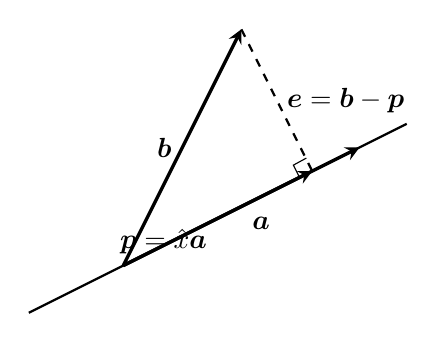
\begin{tikzpicture}[scale=1.5,>=stealth]
			\draw[thick] (-0.8,-0.4) -- (2.4,1.2);
			\draw[->,very thick] (0,0) -- (2,1) node[midway,below right] {$\bm{a}$};
			\draw[->,very thick] (0,0) -- (1,2) node[midway,left] {$\bm{b}$};
			\draw[->,very thick] (0,0) -- (1.6,0.8) node[midway,below left] {$\bm{p}=\hat{x}\bm{a}$};
			\draw[dashed,thick] (1,2) -- (1.6,0.8) node[midway,right] {$\bm{e}=\bm{b}-\bm{p}$};
			\draw (1.49,0.75) -- (1.44,0.85) -- (1.55,0.91);
		\end{tikzpicture}

		图 3：把 $\bm{b}$ 投影到 $\bm{a}$ 张成的直线上
	\end{center}

	直觉已经给出了答案：从 $\bm{b}$ 的终点向直线作垂线，垂足就是最近的点。这个垂足称为 $\bm{b}$ 在这条直线上的\textbf{投影}，记为 $\bm{p}$。下面把 $\bm{p}$ 算出来，每一步都写清楚。

	垂足 $\bm{p}$ 在直线上，所以它是 $\bm{a}$ 的某个倍数：
	\begin{equation}\label{eq:6.19}
	\bm{p}=\hat{x}\bm{a}.
	\end{equation}
	误差向量
	\begin{equation}\label{eq:6.20}
	\bm{e}=\bm{b}-\bm{p}=\bm{b}-\hat{x}\bm{a}
	\end{equation}
	与直线垂直，也就是与 $\bm{a}$ 正交。用点积写出来：
	\begin{equation}\label{eq:6.21}
	\bm{a}\trans(\bm{b}-\hat{x}\bm{a})=0.
	\end{equation}
	把括号分配开：
	\begin{equation}\label{eq:6.22}
	\bm{a}\trans\bm{b}-\hat{x}\,\bm{a}\trans\bm{a}=0.
	\end{equation}
	把含 $\hat{x}$ 的项移到右边：
	\begin{equation}\label{eq:6.23}
	\hat{x}\,\bm{a}\trans\bm{a}=\bm{a}\trans\bm{b}.
	\end{equation}
	因为 $\bm{a}\neq\bm{0}$，$\bm{a}\trans\bm{a}=\norm{\bm{a}}^2$ 是一个正数，可以除过去：
	\begin{equation}\label{eq:6.24}
	\hat{x}=\frac{\bm{a}\trans\bm{b}}{\bm{a}\trans\bm{a}}.
	\end{equation}
代回 $\bm{p}=\hat{x}\bm{a}$，得到投影公式~\eqref{eq:6.25}
	\begin{equation}\label{eq:6.25}
	\boxed{\bm{p}=\frac{\bm{a}\trans\bm{b}}{\bm{a}\trans\bm{a}}\bm{a}.}
	\end{equation}

	拿具体数字算一遍。取
	\begin{equation}\label{eq:6.26}
	\bm{a}=(1,1,1)\trans,
	\qquad
	\bm{b}=(1,2,3)\trans.
	\end{equation}
	先算两个点积：
	\begin{equation}\label{eq:6.27}
	\bm{a}\trans\bm{b}=1+2+3=6,
	\qquad
	\bm{a}\trans\bm{a}=1+1+1=3,
	\end{equation}
	所以
	\begin{equation}\label{eq:6.28}
	\hat{x}=\frac{6}{3}=2,
	\qquad
	\bm{p}=2\bm{a}=(2,2,2)\trans.
	\end{equation}
	误差是
	\begin{equation}\label{eq:6.29}
	\bm{e}=\bm{b}-\bm{p}=(-1,0,1)\trans.
	\end{equation}
	它是否真的与 $\bm{a}$ 垂直？做点积检验：
	\begin{equation}\label{eq:6.30}
	\bm{a}\trans\bm{e}=-1+0+1=0.
	\end{equation}
	确实垂直，答案经得起检查。

再换个角度看公式~\eqref{eq:6.25}。$\bm{a}\trans\bm{b}$ 是标量，可以改变乘法结合的顺序：
	\begin{equation}\label{eq:6.31}
	\bm{p}
	=\bm{a}\,\frac{\bm{a}\trans\bm{b}}{\bm{a}\trans\bm{a}}
	=\frac{\bm{a}\bm{a}\trans}{\bm{a}\trans\bm{a}}\,\bm{b},
	\end{equation}
	这里用到 $\bm{a}(\bm{a}\trans\bm{b})=(\bm{a}\bm{a}\trans)\bm{b}$：左边是向量乘标量，右边是矩阵乘向量，逐分量展开后完全相同。这说明投影是一个矩阵作用在 $\bm{b}$ 上：$\bm{p}=P\bm{b}$，其中
	\begin{equation}\label{eq:6.32}
	\boxed{P=\frac{\bm{a}\bm{a}\trans}{\bm{a}\trans\bm{a}}.}
	\end{equation}
	注意分子 $\bm{a}\bm{a}\trans$ 是 $n\times n$ 矩阵（列乘行），分母 $\bm{a}\trans\bm{a}$ 是标量（行乘列），两者的顺序不能颠倒。

	用上面的例子，$\bm{a}\bm{a}\trans$ 是全 $1$ 矩阵，所以
	\begin{equation}\label{eq:6.33}
	P=\frac{1}{3}
	\begin{bmatrix}
		1&1&1\\
		1&1&1\\
		1&1&1
	\end{bmatrix},
	\qquad
	P\bm{b}
	=\frac{1}{3}
	\begin{bmatrix}
		6\\
		6\\
		6
	\end{bmatrix}
	=
	\begin{bmatrix}
		2\\
		2\\
		2
	\end{bmatrix}
	=\bm{p},
	\end{equation}
与刚才直接代入公式~\eqref{eq:6.25} 的结果一致。

	投影矩阵有两条标志性性质。第一条：
	\begin{equation}\label{eq:6.34}
	P^2=P.
	\end{equation}
直接代入公式~\eqref{eq:6.30} 验证：
	\begin{equation}\label{eq:6.35}
	P^2
	=\frac{\bm{a}\bm{a}\trans}{\bm{a}\trans\bm{a}}\,
	\frac{\bm{a}\bm{a}\trans}{\bm{a}\trans\bm{a}}
	=\frac{\bm{a}\,(\bm{a}\trans\bm{a})\,\bm{a}\trans}{(\bm{a}\trans\bm{a})^2}
	=\frac{\bm{a}\bm{a}\trans}{\bm{a}\trans\bm{a}}
	=P,
	\end{equation}
	中间一步把标量 $\bm{a}\trans\bm{a}$ 约掉了。几何上这很自然：$\bm{p}$ 已经在直线上，再投影一次不会动。第二条：
	\begin{equation}\label{eq:6.36}
	P\trans=P,
	\end{equation}
	因为 $(\bm{a}\bm{a}\trans)\trans=\bm{a}\bm{a}\trans$，转置不改变分子，分母又是标量。正交投影的矩阵一定对称。

	与 $P$ 搭配的还有 $I-P$。它作用在 $\bm{b}$ 上给出
	\begin{equation}\label{eq:6.37}
	(I-P)\bm{b}=\bm{b}-\bm{p}=\bm{e},
	\end{equation}
	即把 $\bm{b}$ 投影到与 $\bm{a}$ 垂直的方向上。$P$ 与 $I-P$ 正好把向量拆成“沿直线”与“垂直直线”两部分。

	\subsection{投影到列空间}

	现在把直线换成一般的列空间。设 $A\in\R^{m\times n}$，并且它的 $n$ 个列向量线性无关——这个条件后面马上会用到，不能丢。给定 $\bm{b}\in\R^m$，要在 $C(A)$ 中找离 $\bm{b}$ 最近的向量，即 $\bm{b}$ 在 $C(A)$ 上的投影。

	列空间里的向量都是列向量的线性组合，也就是某个 $A\hat{\bm{x}}$，所以投影一定可以写成
	\begin{equation}\label{eq:6.38}
	\bm{p}=A\hat{\bm{x}}.
	\end{equation}
	未知量从标量 $\hat{x}$ 变成了向量 $\hat{\bm{x}}$，但投影的条件不变：误差
	\begin{equation}\label{eq:6.39}
	\bm{e}=\bm{b}-A\hat{\bm{x}}
	\end{equation}
	必须垂直于整个列空间。一个向量垂直于列空间，当且仅当它垂直于 $A$ 的每一列——与每列做点积都为零，与它们任意线性组合的点积自然也为零。逐列写出来：
	\begin{equation}\label{eq:6.40}
	\bm{a}_1\trans\bm{e}=0,
	\qquad
	\bm{a}_2\trans\bm{e}=0,
	\ \ldots,\ 
	\bm{a}_n\trans\bm{e}=0,
	\end{equation}
	其中 $\bm{a}_1,\ldots,\bm{a}_n$ 是 $A$ 的各列。把这 $n$ 个等式叠在一起，恰好是
	\begin{equation}\label{eq:6.41}
	A\trans\bm{e}=\bm{0}.
	\end{equation}
	代入 $\bm{e}=\bm{b}-A\hat{\bm{x}}$：
	\begin{equation}\label{eq:6.42}
	A\trans(\bm{b}-A\hat{\bm{x}})=\bm{0}.
	\end{equation}
	分配开再移项：
	\begin{equation}\label{eq:6.43}
	\boxed{A\trans A\hat{\bm{x}}=A\trans\bm{b}.}
	\end{equation}
	这组方程称为\textbf{正规方程}。直线情形是它的特例：当 $A$ 只有一列 $\bm{a}$ 时，$A\trans A=\bm{a}\trans\bm{a}$，$A\trans\bm{b}=\bm{a}\trans\bm{b}$，正规方程就退化成上一节的 $\hat{x}\,\bm{a}\trans\bm{a}=\bm{a}\trans\bm{b}$。

	要从正规方程解出 $\hat{\bm{x}}$，需要 $A\trans A$ 可逆。“列向量线性无关”这个条件正是在这里派上用场。我们验证 $A\trans A$ 的零空间只有零向量：若
	\begin{equation}\label{eq:6.44}
	A\trans A\bm{x}=\bm{0},
	\end{equation}
	两边左乘 $\bm{x}\trans$，得
	\begin{equation}\label{eq:6.45}
	\bm{x}\trans A\trans A\bm{x}=0.
	\end{equation}
	左边结合一下，正好是
	\begin{equation}\label{eq:6.46}
	(A\bm{x})\trans(A\bm{x})=\norm{A\bm{x}}^2.
	\end{equation}
	长度为零的向量只有零向量，所以 $A\bm{x}=\bm{0}$。而列向量线性无关时，$A\bm{x}=\bm{0}$ 只有解 $\bm{x}=\bm{0}$。于是 $A\trans A$ 这个 $n\times n$ 方阵的零空间只有零向量，它可逆。

	因此可以把 $\hat{\bm{x}}$ 解出来：
	\begin{equation}\label{eq:6.47}
	\boxed{\hat{\bm{x}}=(A\trans A)^{-1}A\trans\bm{b}.}
	\end{equation}
	投影向量是
	\begin{equation}\label{eq:6.48}
	\bm{p}=A\hat{\bm{x}}
	=A(A\trans A)^{-1}A\trans\bm{b},
	\end{equation}
	所以投影到 $C(A)$ 的投影矩阵为
	\begin{equation}\label{eq:6.49}
	\boxed{P=A(A\trans A)^{-1}A\trans.}
	\end{equation}
	这里有个常见错误要避开：不能把括号拆开写成 $AA^{-1}(A\trans)^{-1}A\trans=I$，因为 $A$ 一般不是方阵，根本没有逆。

	$P^2=P$ 与 $P\trans=P$ 仍然成立。以 $P^2$ 为例：
	\begin{equation}\label{eq:6.50}
	P^2
	=A(A\trans A)^{-1}A\trans\,A(A\trans A)^{-1}A\trans
	=A(A\trans A)^{-1}\,(A\trans A)\,(A\trans A)^{-1}A\trans,
	\end{equation}
	中间的 $(A\trans A)^{-1}(A\trans A)$ 是单位矩阵，约去后即得 $P^2=P$。对称性同样直接展开验证即可。

	误差落在哪？$\bm{e}=\bm{b}-\bm{p}$ 满足 $A\trans\bm{e}=\bm{0}$，也就是说
	\begin{equation}\label{eq:6.51}
	\bm{e}=\bm{b}-\bm{p}\in N(A\trans).
	\end{equation}
	这与第一节完全一致：$\bm{b}$ 被拆成了列空间里的 $\bm{p}$ 和左零空间里的 $\bm{e}$，两者正交。

	\subsection{最小二乘}

	实际中最常遇到的是方程个数比未知数多的情形：$A\in\R^{m\times n}$，$m>n$。这时
	\begin{equation}\label{eq:6.52}
	A\bm{x}=\bm{b}
	\end{equation}
	通常没有精确解，因为 $C(A)$ 只是 $\R^m$ 中一个 $n$ 维子空间，$\bm{b}$ 多半不在里面。

	无解不等于没办法。$A\bm{x}-\bm{b}$ 的第 $i$ 个分量，就是第 $i$ 个方程“差多少”。这些误差有正有负，直接相加会互相抵消，所以改为最小化误差的平方和：
	\begin{equation}\label{eq:6.53}
	\hat{\bm{x}}
	=
	\arg\min_{\bm{x}}
	\norm{A\bm{x}-\bm{b}}^2.
	\end{equation}
	让误差平方和最小的 $\hat{\bm{x}}$ 称为\textbf{最小二乘解}。

	几何上这个问题已经解决了：$\norm{A\bm{x}-\bm{b}}$ 是 $\bm{b}$ 到列空间中向量 $A\bm{x}$ 的距离，距离最近时 $A\hat{\bm{x}}$ 正是 $\bm{b}$ 在 $C(A)$ 上的投影。于是最佳误差
	\begin{equation}\label{eq:6.54}
	\bm{e}=\bm{b}-A\hat{\bm{x}}
	\end{equation}
	满足 $A\trans\bm{e}=\bm{0}$，再次得到正规方程
	\begin{equation}\label{eq:6.55}
	A\trans A\hat{\bm{x}}=A\trans\bm{b}.
	\end{equation}

	纯代数也能看到同一个结论。固定 $\bm{e}=\bm{b}-A\hat{\bm{x}}$，对任意 $\bm{x}$ 把误差向量拆开：
	\begin{equation}\label{eq:6.56}
	A\bm{x}-\bm{b}
	=A\bm{x}-A\hat{\bm{x}}+A\hat{\bm{x}}-\bm{b}
	=A(\bm{x}-\hat{\bm{x}})-\bm{e}.
	\end{equation}
	前一项 $A(\bm{x}-\hat{\bm{x}})$ 属于 $C(A)$，$\bm{e}$ 属于 $N(A\trans)$，两者正交。正交向量之和的长度平方可以逐项展开，交叉项都是零：
	\begin{equation}\label{eq:6.57}
	\norm{A\bm{x}-\bm{b}}^2
	=\norm{A(\bm{x}-\hat{\bm{x}})}^2+\norm{\bm{e}}^2
	\ge \norm{\bm{e}}^2.
	\end{equation}
	等号成立当且仅当 $A(\bm{x}-\hat{\bm{x}})=\bm{0}$；列向量线性无关时，这等价于 $\bm{x}=\hat{\bm{x}}$。所以正规方程的解确实唯一地给出最小值。

	也可以把目标函数直接展开（这一步以后会有用）：
	\begin{equation}\label{eq:6.58}
	\norm{A\bm{x}-\bm{b}}^2
	=(A\bm{x}-\bm{b})\trans(A\bm{x}-\bm{b})
	=\bm{x}\trans A\trans A\bm{x}
	-2\bm{x}\trans A\trans\bm{b}
	+\bm{b}\trans\bm{b}.
	\end{equation}
	展开时注意 $\bm{b}\trans A\bm{x}$ 与 $\bm{x}\trans A\trans\bm{b}$ 都是标量，且互为转置，所以相等，合并成 $-2\bm{x}\trans A\trans\bm{b}$。

	最经典的应用是直线拟合。给定 $m$ 个数据点 $(t_i,b_i)$，想用一条直线
	\begin{equation}\label{eq:6.59}
	b=C+Dt
	\end{equation}
	尽量经过它们。把每个点代入，得到 $m$ 个方程
	\begin{equation}\label{eq:6.60}
	C+Dt_i=b_i,
	\qquad
	i=1,2,\ldots,m,
	\end{equation}
	写成矩阵形式 $A\bm{x}=\bm{b}$，其中
	\begin{equation}\label{eq:6.61}
	A=
	\begin{bmatrix}
		1&t_1\\
		1&t_2\\
		\vdots&\vdots\\
		1&t_m
	\end{bmatrix},
	\qquad
	\bm{x}=
	\begin{bmatrix}
		C\\
		D
	\end{bmatrix},
	\qquad
	\bm{b}=
	\begin{bmatrix}
		b_1\\
		b_2\\
		\vdots\\
		b_m
	\end{bmatrix}.
	\end{equation}
	只要数据点不恰好共线，这 $m$ 个方程就没有公共解 $(C,D)$，而正规方程给出平方误差最小的那条直线。

	完整算一个例子。取三个数据点
	\begin{equation}\label{eq:6.62}
	(0,1),
	\qquad
	(1,5),
	\qquad
	(2,3).
	\end{equation}
	先确认它们不共线：前两个点确定的直线是 $b=1+4t$，它在 $t=2$ 处给出 $9$，与第三个点的纵坐标 $3$ 不符。于是转向最小二乘。三个方程是
	\begin{equation}\label{eq:6.63}
	C=1,
	\qquad
	C+D=5,
	\qquad
	C+2D=3,
	\end{equation}
	对应
	\begin{equation}\label{eq:6.64}
	A=
	\begin{bmatrix}
		1&0\\
		1&1\\
		1&2
	\end{bmatrix},
	\qquad
	\bm{b}=
	\begin{bmatrix}
		1\\
		5\\
		3
	\end{bmatrix}.
	\end{equation}
	计算 $A\trans A$：用 $A\trans$ 的第一行 $(1,1,1)$ 与第二行 $(0,1,2)$，分别与 $A$ 的两列做点积，
	\begin{equation}\label{eq:6.65}
	A\trans A
	=
	\begin{bmatrix}
		1&1&1\\
		0&1&2
	\end{bmatrix}
	\begin{bmatrix}
		1&0\\
		1&1\\
		1&2
	\end{bmatrix}
	=
	\begin{bmatrix}
		1+1+1&0+1+2\\
		0+1+2&0+1+4
	\end{bmatrix}
	=
	\begin{bmatrix}
		3&3\\
		3&5
	\end{bmatrix}.
	\end{equation}
	再算 $A\trans\bm{b}$：
	\begin{equation}\label{eq:6.66}
	A\trans\bm{b}
	=
	\begin{bmatrix}
		1&1&1\\
		0&1&2
	\end{bmatrix}
	\begin{bmatrix}
		1\\
		5\\
		3
	\end{bmatrix}
	=
	\begin{bmatrix}
		1+5+3\\
		0+5+6
	\end{bmatrix}
	=
	\begin{bmatrix}
		9\\
		11
	\end{bmatrix}.
	\end{equation}
	正规方程是
	\begin{equation}\label{eq:6.67}
	\begin{bmatrix}
		3&3\\
		3&5
	\end{bmatrix}
	\begin{bmatrix}
		C\\
		D
	\end{bmatrix}
	=
	\begin{bmatrix}
		9\\
		11
	\end{bmatrix},
	\qquad
	\text{即}
	\qquad
	3C+3D=9,
	\quad
	3C+5D=11.
	\end{equation}
	第一式除以 $3$ 得 $C+D=3$；第二式减去第一式得 $2D=2$。于是
	\begin{equation}\label{eq:6.68}
	D=1,
	\qquad
	C=2,
	\end{equation}
	最佳直线是 $b=2+t$。

	看看这条直线在三个数据点处的表现。预测值是
	\begin{equation}\label{eq:6.69}
	\bm{p}=A\hat{\bm{x}}
	=
	\begin{bmatrix}
		1&0\\
		1&1\\
		1&2
	\end{bmatrix}
	\begin{bmatrix}
		2\\
		1
	\end{bmatrix}
	=
	\begin{bmatrix}
		2\\
		3\\
		4
	\end{bmatrix},
	\end{equation}
	误差是
	\begin{equation}\label{eq:6.70}
	\bm{e}=\bm{b}-\bm{p}
	=
	\begin{bmatrix}
		1\\
		5\\
		3
	\end{bmatrix}
	-
	\begin{bmatrix}
		2\\
		3\\
		4
	\end{bmatrix}
	=
	\begin{bmatrix}
		-1\\
		2\\
		-1
	\end{bmatrix}.
	\end{equation}
	检验 $\bm{e}$ 是否垂直于 $A$ 的两列：
	\begin{equation}\label{eq:6.71}
	(1,1,1)\cdot\bm{e}=-1+2-1=0,
	\qquad
	(0,1,2)\cdot\bm{e}=0+2-2=0.
	\end{equation}
	都为零，即 $\bm{e}\in N(A\trans)$，与理论一致。这条直线的平方误差是
	\begin{equation}\label{eq:6.72}
	\norm{\bm{e}}^2=(-1)^2+2^2+(-1)^2=6.
	\end{equation}
	回头看，这个例子做的就是一件事：把 $\bm{b}=(1,5,3)\trans$ 投影到 $A$ 的列空间，$\bm{p}$ 是投影，$\bm{e}$ 是落在左零空间里的那一部分。

	\subsection{正交归一基与正交矩阵}

	如果一组向量两两正交，并且长度都是 $1$，很多公式会一下子变简单。满足
	\begin{equation}\label{eq:6.73}
	\bm{q}_i\trans\bm{q}_j
	=
	\begin{cases}
		1,&i=j,\\
		0,&i\neq j
	\end{cases}
	\end{equation}
	的向量组 $\bm{q}_1,\ldots,\bm{q}_n$ 称为\textbf{正交归一}的：$i\neq j$ 那一行说两两正交，$i=j$ 那一行说每个向量与自身的点积为 $1$，即长度都是 $1$。

	把它们并排成矩阵
	\begin{equation}\label{eq:6.74}
	Q=
	\begin{bmatrix}
		\bm{q}_1&\cdots&\bm{q}_n
	\end{bmatrix},
	\end{equation}
	计算 $Q\trans Q$ 的第 $(i,j)$ 个元素：它是 $Q\trans$ 的第 $i$ 行（即 $\bm{q}_i\trans$）与 $Q$ 的第 $j$ 列（即 $\bm{q}_j$）的点积 $\bm{q}_i\trans\bm{q}_j$。由正交归一的定义，这个矩阵对角线上全是 $1$，其余全是 $0$：
	\begin{equation}\label{eq:6.75}
	\boxed{Q\trans Q=I.}
	\end{equation}

	当 $Q$ 是方阵时，这 $n$ 个列向量构成 $\R^n$ 的一组正交归一基。它们必然线性无关：若 $c_1\bm{q}_1+\cdots+c_n\bm{q}_n=\bm{0}$，两边与 $\bm{q}_j$ 做点积，左边只剩 $c_j$，所以每个 $c_j=0$。此时 $Q\trans Q=I$ 意味着 $Q\trans$ 就是 $Q$ 的逆，并且
	\begin{equation}\label{eq:6.76}
	QQ\trans=I,
	\qquad
	\boxed{Q^{-1}=Q\trans.}
	\end{equation}
	满足 $Q^{-1}=Q\trans$ 的方阵称为\textbf{正交矩阵}。求逆变成一次转置，这是正交矩阵最省事的地方。平面上的旋转矩阵就是一个例子：
	\begin{equation}\label{eq:6.77}
	Q=
	\begin{bmatrix}
		\cos\theta&-\sin\theta\\
		\sin\theta&\cos\theta
	\end{bmatrix},
	\qquad
	Q\trans Q=
	\begin{bmatrix}
		\cos^2\theta+\sin^2\theta&0\\
		0&\cos^2\theta+\sin^2\theta
	\end{bmatrix}
	=I.
	\end{equation}

正交归一列让投影公式大幅简化。把一般投影公式~\eqref{eq:6.48} 里的 $A$ 换成 $Q$，正规方程 $Q\trans Q\hat{\bm{x}}=Q\trans\bm{b}$ 的系数矩阵直接就是单位矩阵，于是
	\begin{equation}\label{eq:6.78}
	\hat{\bm{x}}=Q\trans\bm{b},
	\qquad
	\bm{p}=Q\hat{\bm{x}}=QQ\trans\bm{b},
	\qquad
	P=QQ\trans.
	\end{equation}
	完全不需要求逆。而且投影系数 $\hat{x}_i=\bm{q}_i\trans\bm{b}$ 各自独立：第 $i$ 个系数只与第 $i$ 个基向量有关。这就是后面的计算都想办法把基变成正交归一基的原因。

	\subsection{Gram--Schmidt 正交化与 \texorpdfstring{$QR$}{QR} 分解}

	手头一般不会正好有正交归一基。Gram--Schmidt 正交化做的事是：从一组线性无关的向量
	\begin{equation}\label{eq:6.79}
	\bm{a}_1,\bm{a}_2,\ldots,\bm{a}_n
	\end{equation}
	出发，逐个减去“已经在前面各方向上的部分”，造出与原来张成同一子空间的正交归一向量 $\bm{q}_1,\ldots,\bm{q}_n$。

	第一步没有前面的方向可减，直接归一化：
	\begin{equation}\label{eq:6.80}
	\bm{q}_1
	=
	\frac{\bm{a}_1}{\norm{\bm{a}_1}}.
	\end{equation}
第二步，从 $\bm{a}_2$ 中减去它在 $\bm{q}_1$ 方向上的投影。因为 $\norm{\bm{q}_1}=1$，投影公式~\eqref{eq:6.25} 简化成 $(\bm{q}_1\trans\bm{a}_2)\bm{q}_1$，于是
	\begin{equation}\label{eq:6.81}
	\bm{u}_2
	=
	\bm{a}_2
	-(\bm{q}_1\trans\bm{a}_2)\bm{q}_1,
	\qquad
	\bm{q}_2
	=
	\frac{\bm{u}_2}{\norm{\bm{u}_2}}.
	\end{equation}
	验证 $\bm{u}_2$ 确实与 $\bm{q}_1$ 正交：
	\begin{equation}\label{eq:6.82}
	\bm{q}_1\trans\bm{u}_2
	=\bm{q}_1\trans\bm{a}_2-(\bm{q}_1\trans\bm{a}_2)\,\bm{q}_1\trans\bm{q}_1
	=\bm{q}_1\trans\bm{a}_2-\bm{q}_1\trans\bm{a}_2
	=0,
	\end{equation}
	其中用到 $\bm{q}_1\trans\bm{q}_1=1$。

	一般地，第 $k$ 步把 $\bm{a}_k$ 在前面 $k-1$ 个方向上的投影全部减掉：
	\begin{equation}\label{eq:6.83}
	\bm{u}_k
	=
	\bm{a}_k
	-
	\sum_{j=1}^{k-1}
	(\bm{q}_j\trans\bm{a}_k)\bm{q}_j,
	\end{equation}
	再归一化：
	\begin{equation}\label{eq:6.84}
	\bm{q}_k
	=
	\frac{\bm{u}_k}{\norm{\bm{u}_k}}.
	\end{equation}
	$\bm{u}_k$ 与之前的每个 $\bm{q}_j$（$j<k$）都正交：
	\begin{equation}\label{eq:6.85}
	\bm{q}_j\trans\bm{u}_k
	=\bm{q}_j\trans\bm{a}_k-(\bm{q}_j\trans\bm{a}_k)\,\bm{q}_j\trans\bm{q}_j
	=0,
	\end{equation}
	因为和式中除第 $j$ 项外的 $\bm{q}$ 都与 $\bm{q}_j$ 正交，点积后只有第 $j$ 项留下来。$\bm{u}_k$ 也不会是零向量：它是 $\bm{a}_k$ 减去前 $k-1$ 个向量张成空间中的某个向量，而 $\bm{a}_1,\ldots,\bm{a}_k$ 线性无关，$\bm{a}_k$ 不在那个空间里，减完不可能为零，归一化永远不会除以零。这样得到的 $\bm{q}_1,\ldots,\bm{q}_n$ 两两正交归一，并且对每个 $k$，前 $k$ 个 $\bm{q}$ 与前 $k$ 个 $\bm{a}$ 张成同一个子空间。

	用两个具体的三维向量完整算一遍。取
	\begin{equation}\label{eq:6.86}
	\bm{a}_1=
	\begin{bmatrix}
		1\\
		2\\
		2
	\end{bmatrix},
	\qquad
	\bm{a}_2=
	\begin{bmatrix}
		1\\
		1\\
		0
	\end{bmatrix}.
	\end{equation}
	第一步，算 $\bm{a}_1$ 的长度：
	\begin{equation}\label{eq:6.87}
	\norm{\bm{a}_1}^2=1^2+2^2+2^2=9,
	\qquad
	\norm{\bm{a}_1}=3,
	\qquad
	\bm{q}_1=\frac{1}{3}
	\begin{bmatrix}
		1\\
		2\\
		2
	\end{bmatrix}.
	\end{equation}
	第二步，先算投影系数：
	\begin{equation}\label{eq:6.88}
	\bm{q}_1\trans\bm{a}_2
	=\frac{1}{3}(1\cdot1+2\cdot1+2\cdot0)
	=\frac{3}{3}
	=1.
	\end{equation}
	从 $\bm{a}_2$ 中减掉这份投影：
	\begin{equation}\label{eq:6.89}
	\bm{u}_2
	=\bm{a}_2-1\cdot\bm{q}_1
	=
	\begin{bmatrix}
		1\\
		1\\
		0
	\end{bmatrix}
	-
	\begin{bmatrix}
		1/3\\
		2/3\\
		2/3
	\end{bmatrix}
	=
	\begin{bmatrix}
		2/3\\
		1/3\\
		-2/3
	\end{bmatrix}.
	\end{equation}
	再算 $\bm{u}_2$ 的长度：
	\begin{equation}\label{eq:6.90}
	\norm{\bm{u}_2}^2=\frac{4}{9}+\frac{1}{9}+\frac{4}{9}=1,
	\qquad
	\norm{\bm{u}_2}=1,
	\qquad
	\bm{q}_2=\bm{u}_2=
	\begin{bmatrix}
		2/3\\
		1/3\\
		-2/3
	\end{bmatrix}.
	\end{equation}
	最后检验正交性：
	\begin{equation}\label{eq:6.91}
	\bm{q}_1\trans\bm{q}_2
	=\frac{1}{3}\cdot\frac{2}{3}+\frac{2}{3}\cdot\frac{1}{3}+\frac{2}{3}\cdot\left(-\frac{2}{3}\right)
	=\frac{2+2-4}{9}
	=0.
	\end{equation}
	两个向量长度都是 $1$，又互相正交，正交归一化完成。

	Gram--Schmidt 还顺手给出一种矩阵分解。把原向量与新向量分别作为矩阵的列：
	\begin{equation}\label{eq:6.92}
	A=
	\begin{bmatrix}
		\bm{a}_1&\cdots&\bm{a}_n
	\end{bmatrix},
	\qquad
	Q=
	\begin{bmatrix}
		\bm{q}_1&\cdots&\bm{q}_n
	\end{bmatrix}.
	\end{equation}
	把上面的过程反过来看：$\bm{a}_1=\norm{\bm{a}_1}\bm{q}_1$ 只用 $\bm{q}_1$ 表示，$\bm{a}_2=(\bm{q}_1\trans\bm{a}_2)\bm{q}_1+\norm{\bm{u}_2}\bm{q}_2$ 只用 $\bm{q}_1,\bm{q}_2$ 表示，一般地 $\bm{a}_k$ 只用前 $k$ 个 $\bm{q}$ 表示。把这些系数收进一个上三角矩阵 $R$，就有
	\begin{equation}\label{eq:6.93}
	\boxed{A=QR.}
	\end{equation}
	左乘 $Q\trans$，利用 $Q\trans Q=I$，得
	\begin{equation}\label{eq:6.94}
	\boxed{R=Q\trans A.}
	\end{equation}
	这就是 $QR$ 分解。

	用刚才的例子验证。$R$ 的元素是各 $\bm{q}$ 与各 $\bm{a}$ 的点积：
	\begin{equation}\label{eq:6.95}
	R=Q\trans A
	=
	\begin{bmatrix}
		\bm{q}_1\trans\bm{a}_1&\bm{q}_1\trans\bm{a}_2\\
		\bm{q}_2\trans\bm{a}_1&\bm{q}_2\trans\bm{a}_2
	\end{bmatrix}
	=
	\begin{bmatrix}
		3&1\\
		0&1
	\end{bmatrix},
	\end{equation}
	其中 $\bm{q}_1\trans\bm{a}_1=\norm{\bm{a}_1}=3$，$\bm{q}_2\trans\bm{a}_1=0$ 正是刚验证过的正交性，$\bm{q}_2\trans\bm{a}_2=\frac{2}{3}+\frac{1}{3}+0=1$。乘回去检查：第一列 $3\bm{q}_1=\bm{a}_1$；第二列 $1\cdot\bm{q}_1+1\cdot\bm{q}_2=(1/3+2/3,\ 2/3+1/3,\ 2/3-2/3)\trans=(1,1,0)\trans=\bm{a}_2$。$A=QR$ 确实成立。

	$QR$ 分解在最小二乘中特别好用。设 $A=QR$，则
	\begin{equation}\label{eq:6.96}
	A\trans A
	=(QR)\trans(QR)
	=R\trans Q\trans QR
	=R\trans R,
	\end{equation}
	中间用到了 $Q\trans Q=I$。正规方程
	\begin{equation}\label{eq:6.97}
	A\trans A\hat{\bm{x}}=A\trans\bm{b}
	\end{equation}
	于是化为
	\begin{equation}\label{eq:6.98}
	R\trans R\hat{\bm{x}}
	=R\trans Q\trans\bm{b}.
	\end{equation}
	$R$ 的对角元是各步归一化之前的长度 $\norm{\bm{u}_k}$，全都大于零，所以 $R$ 可逆，$R\trans$ 也可逆。两边左乘 $(R\trans)^{-1}$，得到
	\begin{equation}\label{eq:6.99}
	\boxed{R\hat{\bm{x}}=Q\trans\bm{b}.}
	\end{equation}
	右边只是几次点积，左边是上三角方程组，从最后一个未知数开始逐个回代即可。最小二乘就这样化成了一次回代。
	\section{特征值、对角化与正定矩阵}

	前面几章的核心问题是线性方程组 $A\bm{x}=\bm{b}$：已知矩阵 $A$ 和输出 $\bm{b}$，反推输入 $\bm{x}$。这一章换一个角度。把 $A$ 乘在一个向量 $\bm{x}$ 上，得到的 $A\bm{x}$ 通常会转向别的方向；但对某些特殊向量，$A\bm{x}$ 仍停留在原来的方向上，只是被拉长或缩短。这些特殊方向就是本章的主角。沿着它们看，矩阵的作用退化成最简单的“乘上一个数”，矩阵的高次幂、微分方程、二次型的正负这些原本复杂的问题，都会因此变得清楚。

	\subsection{特征值与特征向量}

	设 $A$ 是 $n\times n$ 方阵。若非零向量 $\bm{x}\neq\bm{0}$ 满足
	\begin{equation}\label{eq:7.1}
	A\bm{x}=\lambda\bm{x},
	\end{equation}
	就称 $\bm{x}$ 是 $A$ 的一个\textbf{特征向量}，标量 $\lambda$ 称为对应的\textbf{特征值}。这个等式的意思是：$A$ 作用在 $\bm{x}$ 上，结果仍沿着 $\bm{x}$ 的方向，只是长度被乘上了 $\lambda$。

	这里必须排除零向量。$\bm{x}=\bm{0}$ 时等式 $A\bm{0}=\lambda\bm{0}$ 对任何 $\lambda$ 都成立，它不携带任何方向信息。特征向量讨论的是“方向不变”，所以定义里一开始就要求 $\bm{x}\neq\bm{0}$。

	怎样把特征值找出来？把右边移到左边，并注意 $\lambda\bm{x}=\lambda I\bm{x}$，得
	\begin{equation}\label{eq:7.2}
	(A-\lambda I)\bm{x}=\bm{0}.
	\end{equation}
	我们要求这个齐次方程存在非零解。第 3 章讲过，这类方程有没有非零解，与系数矩阵是否可逆直接相连：要有非零解，$A-\lambda I$ 必须不可逆，也就是行列式为零：
	\begin{equation}\label{eq:7.3}
	\boxed{\det(A-\lambda I)=0.}
	\end{equation}
	这是关于 $\lambda$ 的多项式方程，称为\textbf{特征方程}，左边的多项式称为\textbf{特征多项式}。于是整个计算分两步：先解特征方程得到所有特征值，再对每个特征值解齐次方程 $(A-\lambda I)\bm{x}=\bm{0}$，求出对应的特征向量。

	拿一个 $2\times 2$ 矩阵完整算一遍。设
	\begin{equation}\label{eq:7.4}
	A=
	\begin{bmatrix}
		2&1\\
		1&2
	\end{bmatrix}.
	\end{equation}
	第一步，写出特征多项式。先算
	\begin{equation}\label{eq:7.5}
	A-\lambda I=
	\begin{bmatrix}
		2-\lambda&1\\
		1&2-\lambda
	\end{bmatrix},
	\end{equation}
	于是
	\begin{equation}\label{eq:7.6}
	\det(A-\lambda I)
	=(2-\lambda)^2-1
	=\lambda^2-4\lambda+3.
	\end{equation}
	第二步，解特征方程
	\begin{equation}\label{eq:7.7}
	\lambda^2-4\lambda+3=0.
	\end{equation}
	左边因式分解成 $(\lambda-1)(\lambda-3)$，所以两个特征值为
	\begin{equation}\label{eq:7.8}
	\lambda_1=1,\qquad \lambda_2=3.
	\end{equation}
	第三步，对每个特征值分别解 $(A-\lambda I)\bm{x}=\bm{0}$。

	对 $\lambda_1=1$，系数矩阵是
	\begin{equation}\label{eq:7.9}
	A-I=
	\begin{bmatrix}
		1&1\\
		1&1
	\end{bmatrix},
	\qquad
	\begin{bmatrix}
		1&1\\
		1&1
	\end{bmatrix}
	\begin{bmatrix}
		x_1\\
		x_2
	\end{bmatrix}
	=\bm{0}.
	\end{equation}
	两行给出的是同一个方程 $x_1+x_2=0$，即 $x_2=-x_1$。取 $x_1=1$，得特征向量
	\begin{equation}\label{eq:7.10}
	\bm{x}_1=
	\begin{bmatrix}
		1\\
		-1
	\end{bmatrix}.
	\end{equation}
	对 $\lambda_2=3$，系数矩阵是
	\begin{equation}\label{eq:7.11}
	A-3I=
	\begin{bmatrix}
		-1&1\\
		1&-1
	\end{bmatrix},
	\qquad
	\begin{bmatrix}
		-1&1\\
		1&-1
	\end{bmatrix}
	\begin{bmatrix}
		x_1\\
		x_2
	\end{bmatrix}
	=\bm{0}.
	\end{equation}
	两行都是 $-x_1+x_2=0$，即 $x_2=x_1$。取 $x_1=1$，得
	\begin{equation}\label{eq:7.12}
	\bm{x}_2=
	\begin{bmatrix}
		1\\
		1
	\end{bmatrix}.
	\end{equation}
	最后代回定义验证：
	\begin{equation}\label{eq:7.13}
	A\bm{x}_1=
	\begin{bmatrix}
		2&1\\
		1&2
	\end{bmatrix}
	\begin{bmatrix}
		1\\
		-1
	\end{bmatrix}
	=
	\begin{bmatrix}
		1\\
		-1
	\end{bmatrix}
	=1\cdot\bm{x}_1,
	\qquad
	A\bm{x}_2=
	\begin{bmatrix}
		2&1\\
		1&2
	\end{bmatrix}
	\begin{bmatrix}
		1\\
		1
	\end{bmatrix}
	=
	\begin{bmatrix}
		3\\
		3
	\end{bmatrix}
	=3\bm{x}_2.
	\end{equation}
	两个等式都成立，计算无误。

	注意特征向量并不唯一：$\bm{x}_1$ 的任何非零倍数仍满足 $A\bm{x}=1\cdot\bm{x}$，仍是属于 $\lambda_1=1$ 的特征向量。属于同一特征值的所有特征向量，再添上零向量，构成一个子空间，称为该特征值的\textbf{特征空间}。上例中两个特征空间分别是沿 $(1,-1)$ 与沿 $(1,1)$ 的两条直线。

	有几个基本事实最好一并记住。若 $A$ 是 $n\times n$ 方阵，把重根按次数计入，特征方程一共有 $n$ 个复数根 $\lambda_1,\ldots,\lambda_n$。它们与矩阵本身有两个简洁的联系：
	\begin{equation}\label{eq:7.14}
	\lambda_1+\cdots+\lambda_n
	=\operatorname{tr}(A),
	\end{equation}
	\begin{equation}\label{eq:7.15}
	\lambda_1\lambda_2\cdots\lambda_n
	=\det(A).
	\end{equation}
	其中
	\begin{equation}\label{eq:7.16}
	\operatorname{tr}(A)=a_{11}+\cdots+a_{nn}
	\end{equation}
	是对角线元素之和，称为矩阵的\textbf{迹}。用刚才的例子核对：$1+3=4$，等于迹 $2+2$；$1\times 3=3$，等于行列式 $4-1$。每次算完特征值，用这两条快速检验，能挡掉大部分计算错误。

	由第二条还能看出：$\lambda=0$ 是特征值，当且仅当 $\det(A)=0$，即 $A$ 不可逆。这很直接——$A\bm{x}=0\bm{x}=\bm{0}$ 有非零解，说的就是 $A$ 的零空间里存在非零向量。

	如果 $A$ 是三角矩阵，$A-\lambda I$ 仍是三角矩阵，行列式等于对角线元素的乘积：
	\begin{equation}\label{eq:7.17}
	\det(A-\lambda I)=(a_{11}-\lambda)(a_{22}-\lambda)\cdots(a_{nn}-\lambda).
	\end{equation}
	所以三角矩阵的特征值就是对角线元素，直接读出来即可。

	实矩阵的特征值不一定是实数。例如把平面旋转 $90^\circ$ 的矩阵
	\begin{equation}\label{eq:7.18}
	R=
	\begin{bmatrix}
		0&-1\\
		1&0
	\end{bmatrix},
	\qquad
	\det(R-\lambda I)=\lambda^2+1=0,
	\qquad
	\lambda=\pm i.
	\end{equation}
	几何上也合理：转过 $90^\circ$ 之后，没有任何实向量保持原来的方向，自然没有实特征值。特征值以共轭复数成对出现，在非对称矩阵中并不奇怪。

	也有些矩阵的特征值能从几何意义直接读出。第 6 章的投影矩阵满足
	\begin{equation}\label{eq:7.19}
	P^2=P.
	\end{equation}
	若 $P\bm{x}=\lambda\bm{x}$，两边再作用一次 $P$：
	\begin{equation}\label{eq:7.20}
	\lambda\bm{x}=P\bm{x}=P^2\bm{x}=P(\lambda\bm{x})=\lambda P\bm{x}=\lambda^2\bm{x}.
	\end{equation}
	由于 $\bm{x}\neq\bm{0}$，只能有 $\lambda^2=\lambda$，所以特征值只能是
	\begin{equation}\label{eq:7.21}
	0\quad\text{或}\quad 1.
	\end{equation}
	几何含义同样清楚：列空间中的向量满足 $P\bm{x}=\bm{x}$，对应 $\lambda=1$；零空间中的向量满足 $P\bm{x}=\bm{0}$，对应 $\lambda=0$。

	\subsection{对角化}

	假设 $A$ 有 $n$ 个线性无关的特征向量
	\begin{equation}\label{eq:7.22}
	\bm{x}_1,\ldots,\bm{x}_n,
	\end{equation}
	分别对应特征值
	\begin{equation}\label{eq:7.23}
	\lambda_1,\ldots,\lambda_n.
	\end{equation}
	把这些特征向量按列排成矩阵
	\begin{equation}\label{eq:7.24}
	X=
	\begin{bmatrix}
		\bm{x}_1&\cdots&\bm{x}_n
	\end{bmatrix},
	\end{equation}
	并把特征值放进对角矩阵
	\begin{equation}\label{eq:7.25}
	\Lambda=
	\operatorname{diag}(\lambda_1,\ldots,\lambda_n).
	\end{equation}
	$n$ 个特征方程 $A\bm{x}_i=\lambda_i\bm{x}_i$ 可以合并写成一个矩阵等式
	\begin{equation}\label{eq:7.26}
	AX=X\Lambda.
	\end{equation}
	逐列看就明白了：左边 $AX$ 的第 $i$ 列是 $A\bm{x}_i$；右边 $X\Lambda$ 的第 $i$ 列是 $X$ 的第 $i$ 列乘上 $\Lambda$ 的第 $i$ 个对角元素，即 $\lambda_i\bm{x}_i$。两边第 $i$ 列相等，等式成立。

	由于 $X$ 的列向量线性无关，$X$ 可逆。两边右乘 $X^{-1}$，得
	\begin{equation}\label{eq:7.27}
	\boxed{A=X\Lambda X^{-1}.}
	\end{equation}
	这称为矩阵的\textbf{对角化}：$A$ 被分解成“特征向量矩阵 $\times$ 对角矩阵 $\times$ 特征向量矩阵的逆”。

	先用上一节算好的例子验证一遍。那里
	\begin{equation}\label{eq:7.28}
	X=
	\begin{bmatrix}
		1&1\\
		-1&1
	\end{bmatrix},
	\qquad
	\Lambda=
	\begin{bmatrix}
		1&0\\
		0&3
	\end{bmatrix}.
	\end{equation}
	$X$ 的行列式为 $1-(-1)=2\neq0$，可逆，且
	\begin{equation}\label{eq:7.29}
	X^{-1}=\frac{1}{2}
	\begin{bmatrix}
		1&-1\\
		1&1
	\end{bmatrix}.
	\end{equation}
	逐步乘回去：
	\begin{equation}\label{eq:7.30}
	X\Lambda=
	\begin{bmatrix}
		1&3\\
		-1&3
	\end{bmatrix},
	\qquad
	X\Lambda X^{-1}
	=\frac{1}{2}
	\begin{bmatrix}
		1&3\\
		-1&3
	\end{bmatrix}
	\begin{bmatrix}
		1&-1\\
		1&1
	\end{bmatrix}
	=\frac{1}{2}
	\begin{bmatrix}
		4&2\\
		2&4
	\end{bmatrix}
	=
	\begin{bmatrix}
		2&1\\
		1&2
	\end{bmatrix}
	=A.
	\end{equation}
	分解成立。

	对角化的意义，用“换基”的语言来说最清楚。$\bm{x}_1,\ldots,\bm{x}_n$ 线性无关，所以它们构成 $\R^n$ 的一组基——\textbf{特征向量基}。任何向量 $\bm{u}$ 都能唯一写成
	\begin{equation}\label{eq:7.31}
	\bm{u}=c_1\bm{x}_1+\cdots+c_n\bm{x}_n,
	\end{equation}
	系数 $(c_1,\ldots,c_n)$ 就是 $\bm{u}$ 在这组基下的坐标。让 $A$ 作用上去：
	\begin{equation}\label{eq:7.32}
	A\bm{u}
	=c_1A\bm{x}_1+\cdots+c_nA\bm{x}_n
	=c_1\lambda_1\bm{x}_1+\cdots+c_n\lambda_n\bm{x}_n.
	\end{equation}
	看坐标发生了什么：第 $i$ 个坐标只是从 $c_i$ 变成了 $\lambda_i c_i$。在原来的标准基下，$A$ 把各个方向搅在一起；换到特征向量基之后，每个坐标各自乘上自己的特征值，彼此不再纠缠——这正是一个对角矩阵 $\Lambda$ 所做的事。分解 $A=X\Lambda X^{-1}$ 对应三步：$X^{-1}$ 把标准坐标换算成特征向量基坐标，$\Lambda$ 在新坐标下逐坐标缩放，$X$ 再把结果换回标准坐标。不同特征方向之间彼此解耦，每个方向只被乘上自己的特征值，这就是对角化的几何意义。

	最直接的应用是矩阵幂。先平方：
	\begin{equation}\label{eq:7.33}
	A^2
	=(X\Lambda X^{-1})(X\Lambda X^{-1})
	=X\Lambda^2X^{-1},
	\end{equation}
	中间的 $X^{-1}X=I$ 相互抵消。重复同样的抵消，
	\begin{equation}\label{eq:7.34}
	A^k
	=(X\Lambda X^{-1})^k
	=X\Lambda^kX^{-1},
	\qquad
	\Lambda^k
	=
	\operatorname{diag}(\lambda_1^k,\ldots,\lambda_n^k).
	\end{equation}
	对角矩阵的 $k$ 次幂只是把每个对角元素取 $k$ 次幂，于是 $A^k$ 的计算被化成 $n$ 个数的乘方。对我们的例子，
	\begin{equation}\label{eq:7.35}
	A^k
	=\frac{1}{2}
	\begin{bmatrix}
		1&1\\
		-1&1
	\end{bmatrix}
	\begin{bmatrix}
		1&0\\
		0&3^k
	\end{bmatrix}
	\begin{bmatrix}
		1&-1\\
		1&1
	\end{bmatrix}
	=\frac{1}{2}
	\begin{bmatrix}
		1+3^k&-1+3^k\\
		-1+3^k&1+3^k
	\end{bmatrix}.
	\end{equation}
	代入 $k=1$ 正好还原出 $A$。

	矩阵幂回答了一类离散系统的长期行为。若初始向量
	\begin{equation}\label{eq:7.36}
	\bm{u}_0
	=c_1\bm{x}_1+\cdots+c_n\bm{x}_n,
	\end{equation}
	则递推系统
	\begin{equation}\label{eq:7.37}
	\bm{u}_{k+1}=A\bm{u}_k
	\end{equation}
	的解为
	\begin{equation}\label{eq:7.38}
	\bm{u}_k
	=A^k\bm{u}_0
	=
	\sum_{i=1}^{n}c_i\lambda_i^k\bm{x}_i.
	\end{equation}
	每迭代一次，第 $i$ 个特征方向上的分量就乘一次 $\lambda_i$。因此长期行为由特征值的绝对值控制。若所有
	\begin{equation}\label{eq:7.39}
	|\lambda_i|<1,
	\end{equation}
	则每个分量都衰减到零，从而
	\begin{equation}\label{eq:7.40}
	A^k\to 0;
	\end{equation}
	只要有一个 $|\lambda_i|>1$，对应方向上的分量就会被不断放大。

	并非所有矩阵都能对角化。关键不在于“有 $n$ 个特征值”——计入重数后总有 $n$ 个——而在于有没有 $n$ 个线性无关的特征向量。若 $n$ 个特征值互不相同，对应的特征向量必然线性无关，对角化没有障碍。问题出在重复特征值上：它未必能提供与重复次数一样多的线性无关特征向量。特征值作为特征多项式的根出现的次数称为\textbf{代数重数}，对应特征空间的维数——它实际能提供的线性无关特征向量的个数——称为\textbf{几何重数}。矩阵可对角化，当且仅当每个特征值的几何重数都达到它的代数重数，合起来恰好凑出 $n$ 个线性无关的特征向量。

	若
	\begin{equation}\label{eq:7.41}
	A=BCB^{-1},
	\end{equation}
	则称 $A$ 与 $C$ \textbf{相似}。相似矩阵有相同的特征值：设 $C\bm{x}=\lambda\bm{x}$，令 $\bm{y}=B\bm{x}$，则
	\begin{equation}\label{eq:7.42}
	A\bm{y}=BCB^{-1}B\bm{x}=BC\bm{x}=B(\lambda\bm{x})=\lambda B\bm{x}=\lambda\bm{y},
	\end{equation}
	即 $\lambda$ 也是 $A$ 的特征值，特征向量由 $\bm{x}$ 变成 $B\bm{x}$。相似矩阵表示同一个线性变换在不同基下的矩阵，特征值是变换本身的属性，换基不会改变它。对角化正是要找一个与 $A$ 相似的对角矩阵 $\Lambda$——在特征向量基下，这个变换呈现出最简单的样子。

	\subsection{微分方程与矩阵指数}

	递推 $\bm{u}_{k+1}=A\bm{u}_k$ 描述离散时间的变化，它的连续时间版本是微分方程组
	\begin{equation}\label{eq:7.43}
	\frac{d\bm{u}}{dt}=A\bm{u},
	\end{equation}
	其中 $\bm{u}(t)$ 是随时间演化的向量。一维情形 $du/dt=\lambda u$ 的解是 $u(t)=e^{\lambda t}u(0)$，这提示我们尝试指数形式的解。

	设 $A\bm{x}=\lambda\bm{x}$，取
	\begin{equation}\label{eq:7.44}
	\bm{u}(t)=e^{\lambda t}\bm{x}.
	\end{equation}
	逐项验证它满足方程。左边对 $t$ 求导：
	\begin{equation}\label{eq:7.45}
	\frac{d\bm{u}}{dt}
	=\lambda e^{\lambda t}\bm{x};
	\end{equation}
	右边用特征方程：
	\begin{equation}\label{eq:7.46}
	A\bm{u}(t)
	=e^{\lambda t}A\bm{x}
	=\lambda e^{\lambda t}\bm{x}.
	\end{equation}
	两边相等。因此每个特征向量都给出一个独立的指数解，称为一个\textbf{模式}。一般解是这些模式的叠加：若
	\begin{equation}\label{eq:7.47}
	\bm{u}(0)=c_1\bm{x}_1+\cdots+c_n\bm{x}_n,
	\end{equation}
	则
	\begin{equation}\label{eq:7.48}
	\bm{u}(t)=c_1e^{\lambda_1 t}\bm{x}_1+\cdots+c_ne^{\lambda_n t}\bm{x}_n.
	\end{equation}
	这与离散情形完全平行，只是 $\lambda_i^k$ 换成了 $e^{\lambda_i t}$。

	若 $A=X\Lambda X^{-1}$，这套解可以打包成一个矩阵。模仿 $e^x$ 的泰勒级数，定义\textbf{矩阵指数}
	\begin{equation}\label{eq:7.49}
	e^{At}
	=I+At+\frac{(At)^2}{2!}+\cdots.
	\end{equation}
	把 $(At)^k=A^kt^k=X(\Lambda t)^kX^{-1}$ 代入级数的每一项：
	\begin{equation}\label{eq:7.50}
	e^{At}
	=XX^{-1}+X(\Lambda t)X^{-1}+X\frac{(\Lambda t)^2}{2!}X^{-1}+\cdots.
	\end{equation}
	每一项左边提出 $X$、右边提出 $X^{-1}$，中间恰好又拼成指数级数，于是
	\begin{equation}\label{eq:7.51}
	\boxed{e^{At}=Xe^{\Lambda t}X^{-1},}
	\end{equation}
	其中
	\begin{equation}\label{eq:7.52}
	e^{\Lambda t}
	=
	\operatorname{diag}(e^{\lambda_1t},\ldots,e^{\lambda_nt}).
	\end{equation}
	对角矩阵取指数，只需对每个对角元素分别取指数。初值问题的解由此写成
	\begin{equation}\label{eq:7.53}
	\bm{u}(t)=e^{At}\bm{u}(0).
	\end{equation}

	稳定性同样由特征值决定。若所有特征值都满足
	\begin{equation}\label{eq:7.54}
	\operatorname{Re}(\lambda_i)<0,
	\end{equation}
	则每个模式 $e^{\lambda_i t}$ 都衰减，因而
	\begin{equation}\label{eq:7.55}
	e^{At}\to 0,
	\qquad t\to\infty.
	\end{equation}
	这里要看实部，是因为特征值可能是复数。本章一直在用的矩阵特征值为 $1$ 与 $3$，模式 $e^{t}$ 与 $e^{3t}$ 都在增长，对应的系统不稳定。离散与连续两个判据放在一起很整齐：离散系统要 $|\lambda_i|<1$，连续系统要 $\operatorname{Re}(\lambda_i)<0$。

	\subsection{对称矩阵与谱定理}

	对称矩阵
	\begin{equation}\label{eq:7.56}
	S\trans=S
	\end{equation}
	在特征值理论中具有特别整齐的结构：
	\begin{enumerate}
		\item 所有特征值都为实数；
		\item 可以选取一组正交归一的特征向量作为整个 $\R^n$ 的基。
	\end{enumerate}
	第二条中“正交归一”的意思是：任意两个不同的特征向量点积为零，且每个特征向量的长度为一。

	把这样一组单位特征向量按列排成矩阵
	\begin{equation}\label{eq:7.57}
	Q=
	\begin{bmatrix}
		\bm{q}_1&\cdots&\bm{q}_n
	\end{bmatrix}.
	\end{equation}
	列与列正交、长度都为一，用矩阵乘法写出来恰好是
	\begin{equation}\label{eq:7.58}
	Q\trans Q=QQ\trans=I,
	\end{equation}
	这样的矩阵称为\textbf{正交矩阵}，它的逆就是转置：$Q^{-1}=Q\trans$。令
	\begin{equation}\label{eq:7.59}
	\Lambda=\operatorname{diag}(\lambda_1,\ldots,\lambda_n),
	\end{equation}
一般对角化公式~\eqref{eq:7.27} 中的 $X^{-1}$ 于是简化成 $Q\trans$：
	\begin{equation}\label{eq:7.60}
	\boxed{S=Q\Lambda Q\trans.}
	\end{equation}
	这就是实对称矩阵的\textbf{谱定理}，“谱”指特征值的全体。

	与一般的
	\begin{equation}\label{eq:7.61}
	A=X\Lambda X^{-1}
	\end{equation}
	相比，对称矩阵把 $X^{-1}$ 简化成了 $Q\trans$。从几何上可以把
	\begin{equation}\label{eq:7.62}
	S=Q\Lambda Q\trans
	\end{equation}
	读成三步：先用 $Q\trans$ 旋转到特征向量坐标系，再沿各个特征方向按 $\lambda_i$ 缩放，最后用 $Q$ 旋转回来。旋转不改变长度与角度，所以对称矩阵的全部作用，本质上就是沿一组互相垂直的方向各自缩放。

	为什么不同特征值对应的特征向量必然正交？设
	\begin{equation}\label{eq:7.63}
	S\bm{x}=\lambda\bm{x},\qquad S\bm{y}=\mu\bm{y},\qquad \lambda\neq\mu.
	\end{equation}
	用两种方式计算 $\bm{y}\trans S\bm{x}$。先把 $S\bm{x}=\lambda\bm{x}$ 代入：
	\begin{equation}\label{eq:7.64}
	\bm{y}\trans S\bm{x}=\lambda\,\bm{y}\trans\bm{x}.
	\end{equation}
	再利用对称性把 $S$ 挪到 $\bm{y}$ 上：由 $\bm{y}\trans S=(S\bm{y})\trans=(\mu\bm{y})\trans=\mu\bm{y}\trans$，得
	\begin{equation}\label{eq:7.65}
	\bm{y}\trans S\bm{x}=\mu\,\bm{y}\trans\bm{x}.
	\end{equation}
	两式相减，
	\begin{equation}\label{eq:7.66}
	(\lambda-\mu)\,\bm{y}\trans\bm{x}=0.
	\end{equation}
	因为 $\lambda\neq\mu$，只能有 $\bm{y}\trans\bm{x}=0$，即 $\bm{x}$ 与 $\bm{y}$ 正交。

	即使某个特征值重复出现，也可以在它的特征空间内部选一组正交归一基。因此任何实对称矩阵都一定可以正交对角化。

	本章的例子正好是对称矩阵，可以直接看到这一切。两个特征向量 $(1,-1)$ 与 $(1,1)$ 的点积为 $1-1=0$，天然正交；各除以长度 $\sqrt{2}$ 归一化，得
	\begin{equation}\label{eq:7.67}
	\bm{q}_1=\frac{1}{\sqrt{2}}
	\begin{bmatrix}
		1\\
		-1
	\end{bmatrix},
	\qquad
	\bm{q}_2=\frac{1}{\sqrt{2}}
	\begin{bmatrix}
		1\\
		1
	\end{bmatrix},
	\qquad
	Q=\frac{1}{\sqrt{2}}
	\begin{bmatrix}
		1&1\\
		-1&1
	\end{bmatrix}.
	\end{equation}
	谱定理给出分解
	\begin{equation}\label{eq:7.68}
	\begin{bmatrix}
		2&1\\
		1&2
	\end{bmatrix}
	=Q
	\begin{bmatrix}
		1&0\\
		0&3
	\end{bmatrix}
	Q\trans.
	\end{equation}
	把右边乘开，可以验证它确实等于左边的矩阵。

	\subsection{正定矩阵}

	在对称矩阵中，若所有特征值都为正数，则称矩阵 $S$ \textbf{正定}。正定性有几种彼此等价的重要判据：
	\begin{equation}\label{eq:7.69}
	\boxed{
		\begin{aligned}
			&S\text{ 对称且所有特征值 }\lambda_i>0\\
			\Longleftrightarrow\;&S\text{ 的所有主元都为正}\\
			\Longleftrightarrow\;&S\text{ 的所有顺序左上主子式都为正}\\
			\Longleftrightarrow\;&\bm{x}\trans S\bm{x}>0\quad(\bm{x}\neq\bm{0}).
		\end{aligned}}
	\end{equation}
	主元是消元后留在对角线上的那些数（第 4 章）；第 $k$ 个\textbf{顺序左上主子式}是左上角 $k\times k$ 子矩阵的行列式。最后一条称为\textbf{能量判据}，它把正定性说成：任何非零向量带来的“能量” $\bm{x}\trans S\bm{x}$ 都严格为正。

	四条判据说的是同一件事，但验算的难度各不相同。用本章反复出现的矩阵
	\begin{equation}\label{eq:7.70}
	S=
	\begin{bmatrix}
		2&1\\
		1&2
	\end{bmatrix}
	\end{equation}
	逐条验证一遍。

	第一条，特征值。第一节已经算出 $\lambda_1=1$、$\lambda_2=3$，都为正，通过。

	第二条，主元。做一次消元：第二行减去第一行的 $\frac{1}{2}$ 倍，
	\begin{equation}\label{eq:7.71}
	\begin{bmatrix}
		2&1\\
		1&2
	\end{bmatrix}
	\longrightarrow
	\begin{bmatrix}
		2&1\\
		0&\frac{3}{2}
	\end{bmatrix}.
	\end{equation}
	两个主元 $2$ 与 $\frac{3}{2}$ 都为正，通过。

	第三条，顺序左上主子式。一阶主子式是左上角元素 $2>0$；二阶主子式是整个行列式 $2\cdot2-1\cdot1=3>0$，通过。

	第四条，能量判据。设 $\bm{x}=(x_1,x_2)\trans$，逐步行列相乘：
	\begin{equation}\label{eq:7.72}
	\bm{x}\trans S\bm{x}
	=
	\begin{bmatrix}
		x_1&x_2
	\end{bmatrix}
	\begin{bmatrix}
		2x_1+x_2\\
		x_1+2x_2
	\end{bmatrix}
	=2x_1^2+2x_1x_2+2x_2^2.
	\end{equation}
	关键一步是配方：
	\begin{equation}\label{eq:7.73}
	2x_1^2+2x_1x_2+2x_2^2
	=x_1^2+x_2^2+(x_1+x_2)^2.
	\end{equation}
	右边是三个平方之和，永远非负；要让它等于零，必须 $x_1=0$ 且 $x_2=0$，即 $\bm{x}=\bm{0}$。所以只要 $\bm{x}\neq\bm{0}$，就有 $\bm{x}\trans S\bm{x}>0$，通过。

	四条判据全部满足，$S$ 是正定的。由于它们彼此等价，实际判别时任选最方便的一条即可。

	对于一般的二维对称矩阵
	\begin{equation}\label{eq:7.74}
	S=
	\begin{bmatrix}
		a&b\\
		b&c
	\end{bmatrix},
	\end{equation}
	第三条判据给出最常用的快速判别法：
	\begin{equation}\label{eq:7.75}
	\boxed{a>0,\qquad ac-b^2>0.}
	\end{equation}
	这里第一个条件保证第一个主元为正，第二个条件就是行列式为正。也可以从主元看：消元后第二个主元是 $c-\frac{b^2}{a}=\frac{ac-b^2}{a}$，在 $a>0$ 的前提下它为正当且仅当 $ac-b^2>0$。上面的例子中 $a=2>0$、$ac-b^2=3>0$，与逐条验证的结论一致。

	正定矩阵与第 6 章的最小二乘自然联系起来。对任意矩阵 $A$（不必是方阵），
	\begin{equation}\label{eq:7.76}
	A\trans A
	\end{equation}
	一定是对称的，因为 $(A\trans A)\trans=A\trans A$。再看它的能量：
	\begin{equation}\label{eq:7.77}
	\bm{x}\trans A\trans A\bm{x}
	=(A\bm{x})\trans(A\bm{x})
	=\norm{A\bm{x}}^2
	\ge 0.
	\end{equation}
	长度平方不可能为负，所以 $A\trans A$ 总是\textbf{半正定}——对称、且特征值都大于或等于零。什么时候能升级成正定？若 $A$ 的列向量线性无关，则
	\begin{equation}\label{eq:7.78}
	A\bm{x}=\bm{0}
	\end{equation}
	只有零解，于是对所有 $\bm{x}\neq\bm{0}$ 都有
	\begin{equation}\label{eq:7.79}
	\norm{A\bm{x}}^2>0,
	\end{equation}
	从而
	\begin{equation}\label{eq:7.80}
	\boxed{A\trans A\text{ 正定}.}
	\end{equation}
	这也解释了为什么满列秩时正规方程中的 $A\trans A$ 一定可逆：正定矩阵特征值全为正，行列式等于它们的乘积，不可能为零。

	半正定与正定只差在零上。半正定允许
	\begin{equation}\label{eq:7.81}
	\bm{x}\trans S\bm{x}=0
	\end{equation}
	在某些非零方向上出现，也就是特征值可以取零；正定排除了这些“平坦”方向，任何非零方向上的能量都严格为正。

	由谱分解
	\begin{equation}\label{eq:7.82}
	S=Q\Lambda Q\trans
	\end{equation}
	可得
	\begin{equation}\label{eq:7.83}
	\bm{x}\trans S\bm{x}
	=
	(Q\trans\bm{x})\trans
	\Lambda
	(Q\trans\bm{x}).
	\end{equation}
	若令
	\begin{equation}\label{eq:7.84}
	\bm{y}=Q\trans\bm{x},
	\end{equation}
	即把 $\bm{x}$ 旋转到特征向量坐标系，则
	\begin{equation}\label{eq:7.85}
	\bm{x}\trans S\bm{x}
	=
	\lambda_1y_1^2+\cdots+\lambda_ny_n^2.
	\end{equation}
	$\bm{x}\trans S\bm{x}$ 这种每一项都是二次的表达式称为\textbf{二次型}。在特征向量坐标系下，二次型没有交叉项，只是各坐标平方的加权和，权重就是特征值。所以所有 $\lambda_i>0$ 时，除 $\bm{x}=\bm{0}$ 外该二次型始终为正——这正是能量判据与特征值判据等价的原因。

	几何上，方程
	\begin{equation}\label{eq:7.86}
	\bm{x}\trans S\bm{x}=1
	\end{equation}
	描述一个椭球，其主轴方向就是 $S$ 的特征向量，主轴长度与 $1/\sqrt{\lambda_i}$ 成正比。用我们的例子，方程
	\begin{equation}\label{eq:7.87}
	2x_1^2+2x_1x_2+2x_2^2=1
	\end{equation}
	是一个椭圆：沿 $(1,-1)$ 方向的半轴长为 $1/\sqrt{\lambda_1}=1$，沿 $(1,1)$ 方向的半轴长为 $1/\sqrt{\lambda_2}=1/\sqrt{3}$。特征值越大，对应方向被压得越短。

	对称正定矩阵还可以从消元得到
	\begin{equation}\label{eq:7.88}
	S=LDL\trans,
	\end{equation}
	其中 $D$ 的对角元素就是正主元；也可以从特征分解得到
	\begin{equation}\label{eq:7.89}
	S=Q\Lambda Q\trans,
	\end{equation}
	其中 $\Lambda$ 的对角元素就是正特征值。这两个分解分别从消元和特征方向刻画了同一个正定结构。

\end{document}
